%%
%% This is file `sample-sigconf.tex',
%% generated with the docstrip utility.
%%
%% The original source files were:
%%
%% samples.dtx  (with options: `all,proceedings,bibtex,sigconf')
%% 
%% IMPORTANT NOTICE:
%% 
%% For the copyright see the source file.
%% 
%% Any modified versions of this file must be renamed
%% with new filenames distinct from sample-sigconf.tex.
%% 
%% For distribution of the original source see the terms
%% for copying and modification in the file samples.dtx.
%% 
%% This generated file may be distributed as long as the
%% original source files, as listed above, are part of the
%% same distribution. (The sources need not necessarily be
%% in the same archive or directory.)
%%
%%
%% Commands for TeXCount
%TC:macro \cite [option:text,text]
%TC:macro \citep [option:text,text]
%TC:macro \citet [option:text,text]
%TC:envir table 0 1
%TC:envir table* 0 1
%TC:envir tabular [ignore] word
%TC:envir displaymath 0 word
%TC:envir math 0 word
%TC:envir comment 0 0
%%
%%
%% The first command in your LaTeX source must be the \documentclass
%% command.
%%
%% For submission and review of your manuscript please change the
%% command to \documentclass[manuscript, screen, review]{acmart}.
%%
%% When submitting camera ready or to TAPS, please change the command
%% to \documentclass[sigconf]{acmart} or whichever template is required
%% for your publication.
%%
%%
\documentclass[sigconf]{acmart}
\graphicspath{{images/}}
\usepackage{subcaption}
\usepackage{xcolor} % import color package
\newcommand{\specialterm}[1]{\textcolor{blue}{#1}}
%%
%% \BibTeX command to typeset BibTeX logo in the docs
\AtBeginDocument{%
  \providecommand\BibTeX{{%
    Bib\TeX}}}

%% Rights management information.  This information is sent to you
%% when you complete the rights form.  These commands have SAMPLE
%% values in them; it is your responsibility as an author to replace
%% the commands and values with those provided to you when you
%% complete the rights form.
% \setcopyright{acmlicensed}
% \copyrightyear{2018}
% \acmYear{2018}
% \acmDOI{XXXXXXX.XXXXXXX}

%% These commands are for a PROCEEDINGS abstract or paper.
% \acmConference[Conference acronym 'XX]{Make sure to enter the correct
%   conference title from your rights confirmation emai}{June 03--05,
%   2018}{Woodstock, NY}
%%
%%  Uncomment \acmBooktitle if the title of the proceedings is different
%%  from ``Proceedings of ...''!
%%
%%\acmBooktitle{Woodstock '18: ACM Symposium on Neural Gaze Detection,
%%  June 03--05, 2018, Woodstock, NY}
% \acmISBN{978-1-4503-XXXX-X/18/06}


%%
%% Submission ID.
%% Use this when submitting an article to a sponsored event. You'll
%% receive a unique submission ID from the organizers
%% of the event, and this ID should be used as the parameter to this command.
%%\acmSubmissionID{123-A56-BU3}

%%
%% For managing citations, it is recommended to use bibliography
%% files in BibTeX format.
%%
%% You can then either use BibTeX with the ACM-Reference-Format style,
%% or BibLaTeX with the acmnumeric or acmauthoryear sytles, that include
%% support for advanced citation of software artefact from the
%% biblatex-software package, also separately available on CTAN.
%%
%% Look at the sample-*-biblatex.tex files for templates showcasing
%% the biblatex styles.
%%

%%
%% The majority of ACM publications use numbered citations and
%% references.  The command \citestyle{authoryear} switches to the
%% "author year" style.
%%
%% If you are preparing content for an event
%% sponsored by ACM SIGGRAPH, you must use the "author year" style of
%% citations and references.
%% Uncommenting
%% the next command will enable that style.
%%\citestyle{acmauthoryear}


%%
%% end of the preamble, start of the body of the document source.
\begin{document}

%%
%% The "title" command has an optional parameter,
%% allowing the author to define a "short title" to be used in page headers.
\title{Developing an Android Application for SplitMateEZ}

%%
%% The "author" command and its associated commands are used to define
%% the authors and their affiliations.
%% Of note is the shared affiliation of the first two authors, and the
%% "authornote" and "authornotemark" commands
%% used to denote shared contribution to the research.
\author{Zuxing Wu}
\email{a1816653@adelaide.edu.au}
\affiliation{%
  \institution{University of Adelaide}
  \city{Adelaide}
  \state{SA}
  \country{Australia}
}

%%
%% By default, the full list of authors will be used in the page
%% headers. Often, this list is too long, and will overlap
%% other information printed in the page headers. This command allows
%% the author to define a more concise list
%% of authors' names for this purpose.
\renewcommand{\shortauthors}{Zuxing Wu}

%%
%% The abstract is a short summary of the work to be presented in the
%% article.
\begin{abstract}
  This part will be written after the completion of the paper.
\end{abstract}

%%
%% The code below is generated by the tool at http://dl.acm.org/ccs.cfm.
%% Please copy and paste the code instead of the example below.
%%
% \begin{CCSXML}
% <ccs2012>
%  <concept>
%   <concept_id>00000000.0000000.0000000</concept_id>
%   <concept_desc>Do Not Use This Code, Generate the Correct Terms for Your Paper</concept_desc>
%   <concept_significance>500</concept_significance>
%  </concept>
%  <concept>
%   <concept_id>00000000.00000000.00000000</concept_id>
%   <concept_desc>Do Not Use This Code, Generate the Correct Terms for Your Paper</concept_desc>
%   <concept_significance>300</concept_significance>
%  </concept>
%  <concept>
%   <concept_id>00000000.00000000.00000000</concept_id>
%   <concept_desc>Do Not Use This Code, Generate the Correct Terms for Your Paper</concept_desc>
%   <concept_significance>100</concept_significance>
%  </concept>
%  <concept>
%   <concept_id>00000000.00000000.00000000</concept_id>
%   <concept_desc>Do Not Use This Code, Generate the Correct Terms for Your Paper</concept_desc>
%   <concept_significance>100</concept_significance>
%  </concept>
% </ccs2012>
% \end{CCSXML}

% \ccsdesc[500]{Do Not Use This Code~Generate the Correct Terms for Your Paper}
% \ccsdesc[300]{Do Not Use This Code~Generate the Correct Terms for Your Paper}
% \ccsdesc{Do Not Use This Code~Generate the Correct Terms for Your Paper}
% \ccsdesc[100]{Do Not Use This Code~Generate the Correct Terms for Your Paper}

%%
%% Keywords. The author(s) should pick words that accurately describe
%% the work being presented. Separate the keywords with commas.
\keywords{Android Application, Shared Accommodation, Bills Splitting, Large Language Models, IoT, Usage Tracking, Face Recognition, Text Recognition}
%% A "teaser" image appears between the author and affiliation
%% information and the body of the document, and typically spans the
%% page.
% \begin{teaserfigure}
%   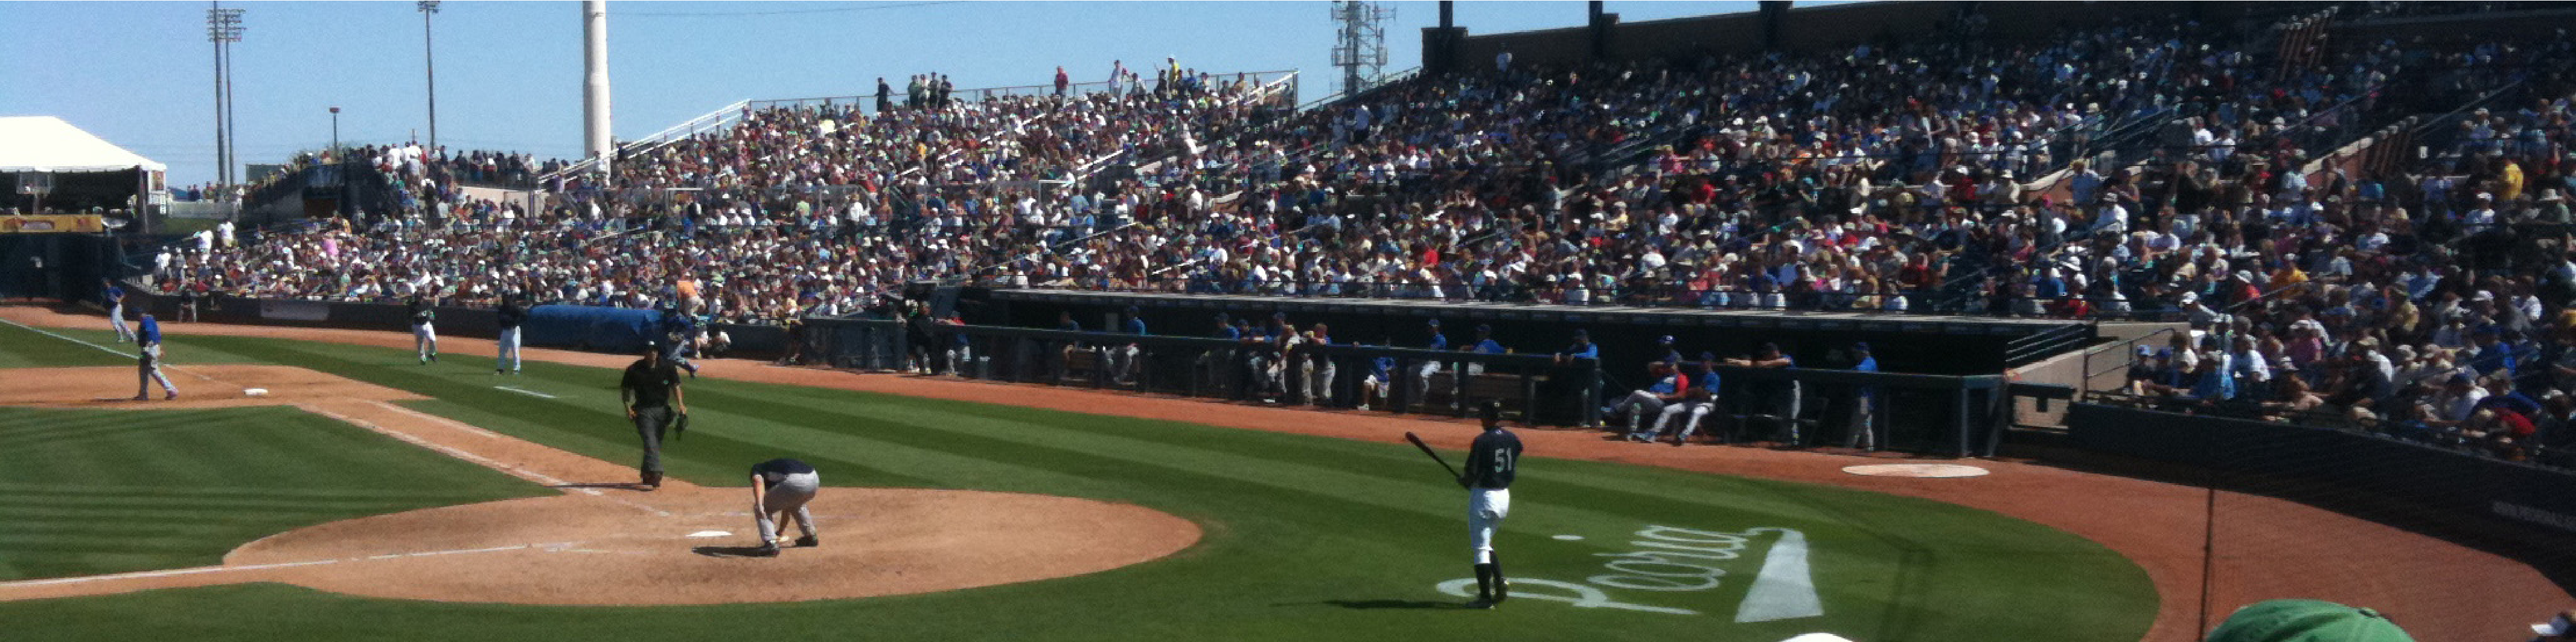
\includegraphics[width=\textwidth]{sampleteaser}
%   \caption{Seattle Mariners at Spring Training, 2010.}
%   \Description{Enjoying the baseball game from the third-base
%   seats. Ichiro Suzuki preparing to bat.}
%   \label{fig:teaser}
% \end{teaserfigure}

% \received{20 February 2007}
% \received[revised]{12 March 2009}
% \received[accepted]{5 June 2009}

%%
%% This command processes the author and affiliation and title
%% information and builds the first part of the formatted document.
\maketitle

\section{Introduction}
In shared accommodations, dividing utility bills among roommates often proves to be a complex and contentious issue. Many current solutions for bill-splitting rely on estimations and manual reporting, which can lead to discrepancies and disputes among residents. The implementation of SplitMateEZ system addresses this problem by leveraging the latest advancements in Internet of Things (IoT) technology, security cameras, and Large Language Models (LLMs) to provide a more accurate and efficient solution for bill-splitting.  

SplitMateEZ offers a user-friendly Android application that allows residents to monitor their utility usage, receive real-time notifications, and access detailed reports. The system uses security cameras to track residents' movements and activities, which are then analyzed by LLMs to determine the amount of time each resident spends in resource areas. This data is used to calculate each resident's share of the utility bills, ensuring a fair and transparent distribution of costs. SplitMateEZ also provides a platform for residents to communicate and resolve any disputes that may arise, promoting a harmonious living environment.

\section{Motivation}
The biggest problem of splitting bills in shared accommodations is the lack of usage tracking. With cameras and Cloud sever, we can store the captured data and analyze it to determine the amount of time each resident spends in different resources. This data is used to calculate each resident's share of the utility bills, ensuring a fair and transparent distribution of costs. The data can also be used to generate detailed reports and provide insights into residents' usage patterns, helping them to identify areas where they can reduce their consumption and save money.  

The data collection and data storage parts are done by my two teammates. I am responsible for developing the Android application that will be used by residents to display their usage data, receive notifications, and communicate with other residents, etc.

\section{Existing Work}

\section{My Work}
My part in this project is to develop an Android application that will be used by residents to check their usage data, receive notifications, pay bills, and communicate with other residents living in the same house. The application will have
some basic functions such as: 
\begin{enumerate}
  \item \textbf{User authentication}: Users can log in to the application using their email address and password.
  \item \textbf{Notifications}: Residents will receive real-time notifications about their unpaid bills or stangers trespassing. 
  \item \textbf{Communication}: Landlord can communicate with all residents, and residents can only talk to the landlord. 
  \item \textbf{Management}: Landlord can add new properties and add new tenants into a property.
\end{enumerate}

Besides these basic functions, I also implemented some specialized functions including: 
\begin{enumerate}
  \item \textbf{Face recognition}: Tennats can only upload their profile photo through phone camera and ensure there is a face in that photo, otherwise they have no access to other pages.
  \item \textbf{Text recognition}: Landlords can take a photo of their bills, and the application will automatically extract the information from the photo and save it into the system for the bill Splitting.
  \item \textbf{Usage tracking}: All residents can view their usage data for different resources, such as electricity, water, Internet, and gas. It will show the total usage durations for each resource in a day, a week, or a month.
  \item \textbf{Actions history}: All residents can view their actions history from a continuous timeline interface.
  \item \textbf{Pay bills}: Residents can pay their bills through the application.
  \item \textbf{Generate Report}: Residents can generate a monthly usage report for their usage data and can also get some insights or recommendations from it.
\end{enumerate}


\section{Results}
Aforementioned functions have been implemented in the SplitMateEZ Android application. The application has been tested on two different models of Android phones and is working as expected. The application is user-friendly and provides a seamless experience for residents to chack their usage logs, pay their bills and communicate with their landlord.
\subsection{Basic Functions}
\subsubsection{User Authentication}
The user authentication function allows residents to log in to the application using their email address and password (Figure~\ref{fig:logIn}). Email address is required for the registration (Figure~\ref{fig:signUp}). Users can sign up as a tenant or a landlord if they are the owner of the property.
The application verifies the user's credentials and grants access to the user's account if the credentials are correct. If the credentials are incorrect, the application displays an error message and prompts the user to enter the correct information.
\begin{figure}[h]
  \centering
  \begin{subfigure}{0.24\textwidth}
    \raggedright
    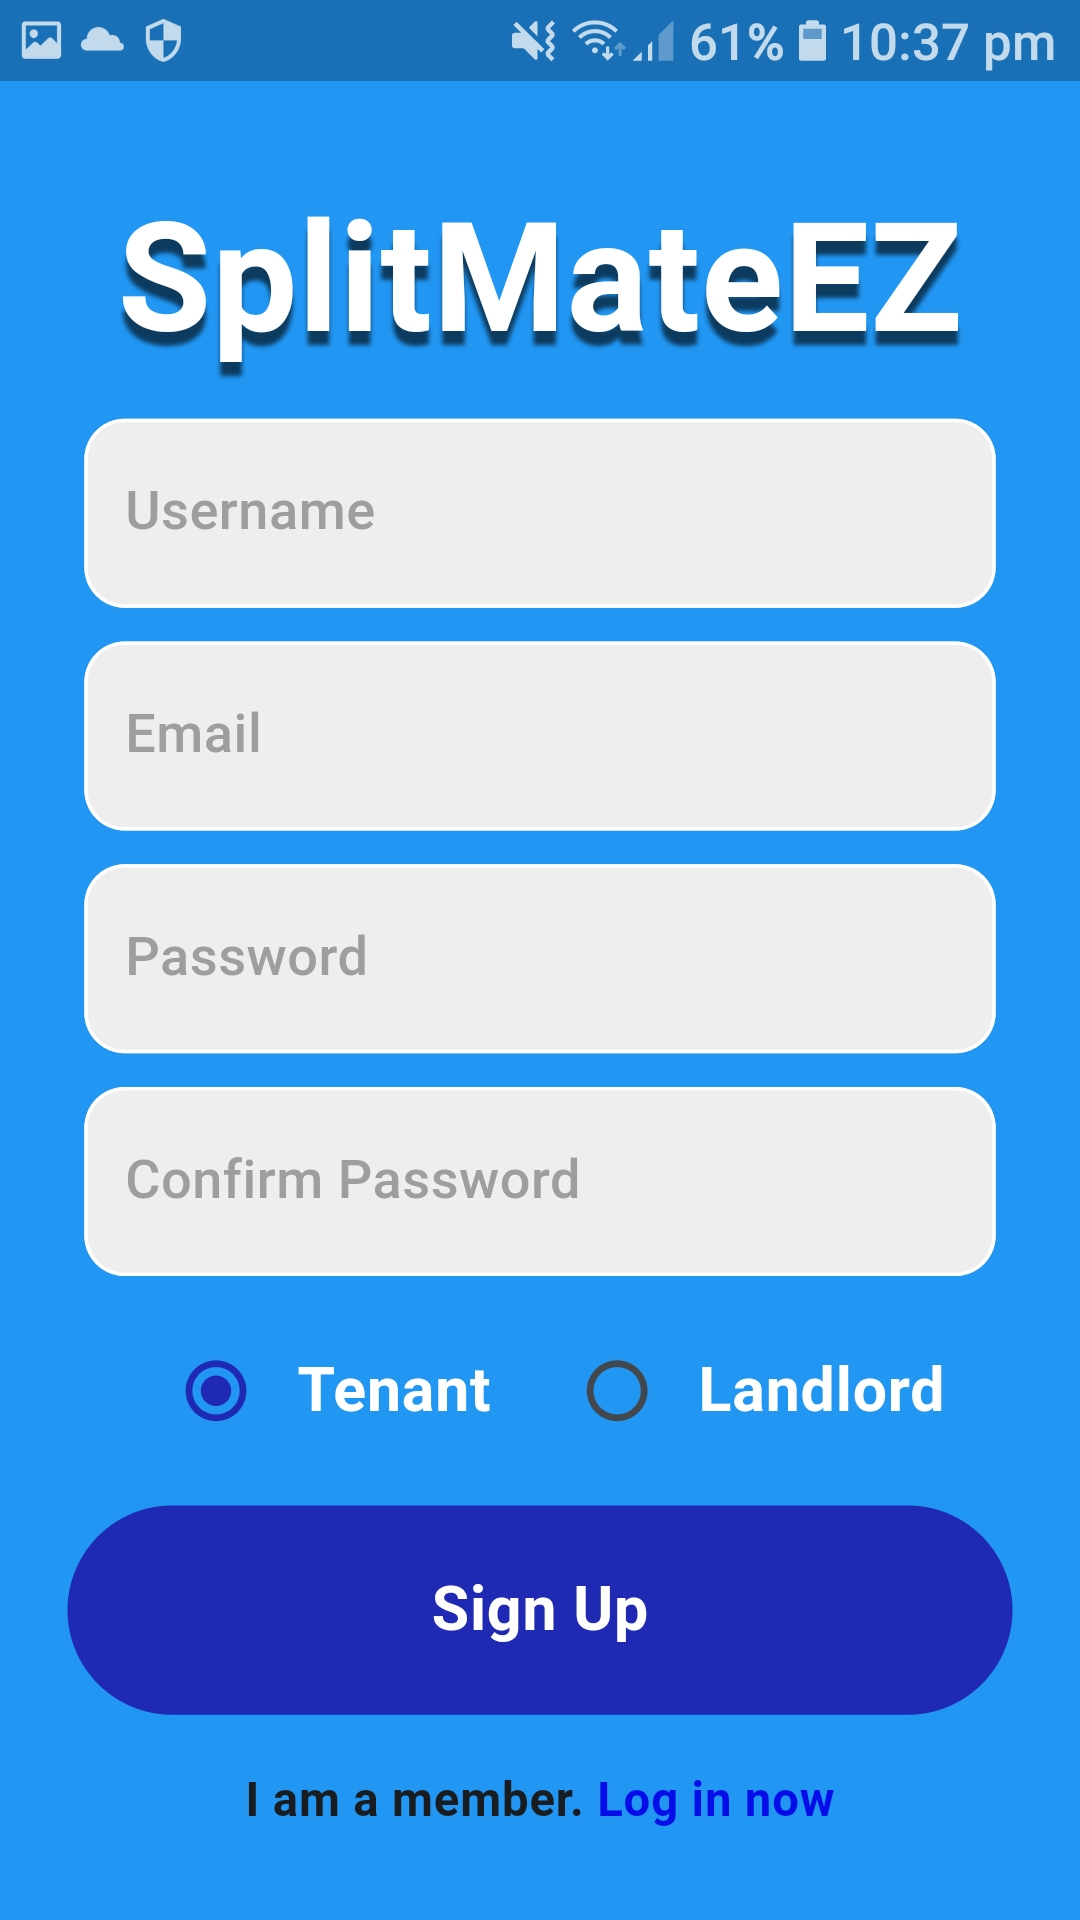
\includegraphics[width=\linewidth]{signUp.jpg}
    \caption{Sign Up Page}
    \label{fig:signUp}
  \end{subfigure}
  \begin{subfigure}{0.24\textwidth}
    \raggedleft
    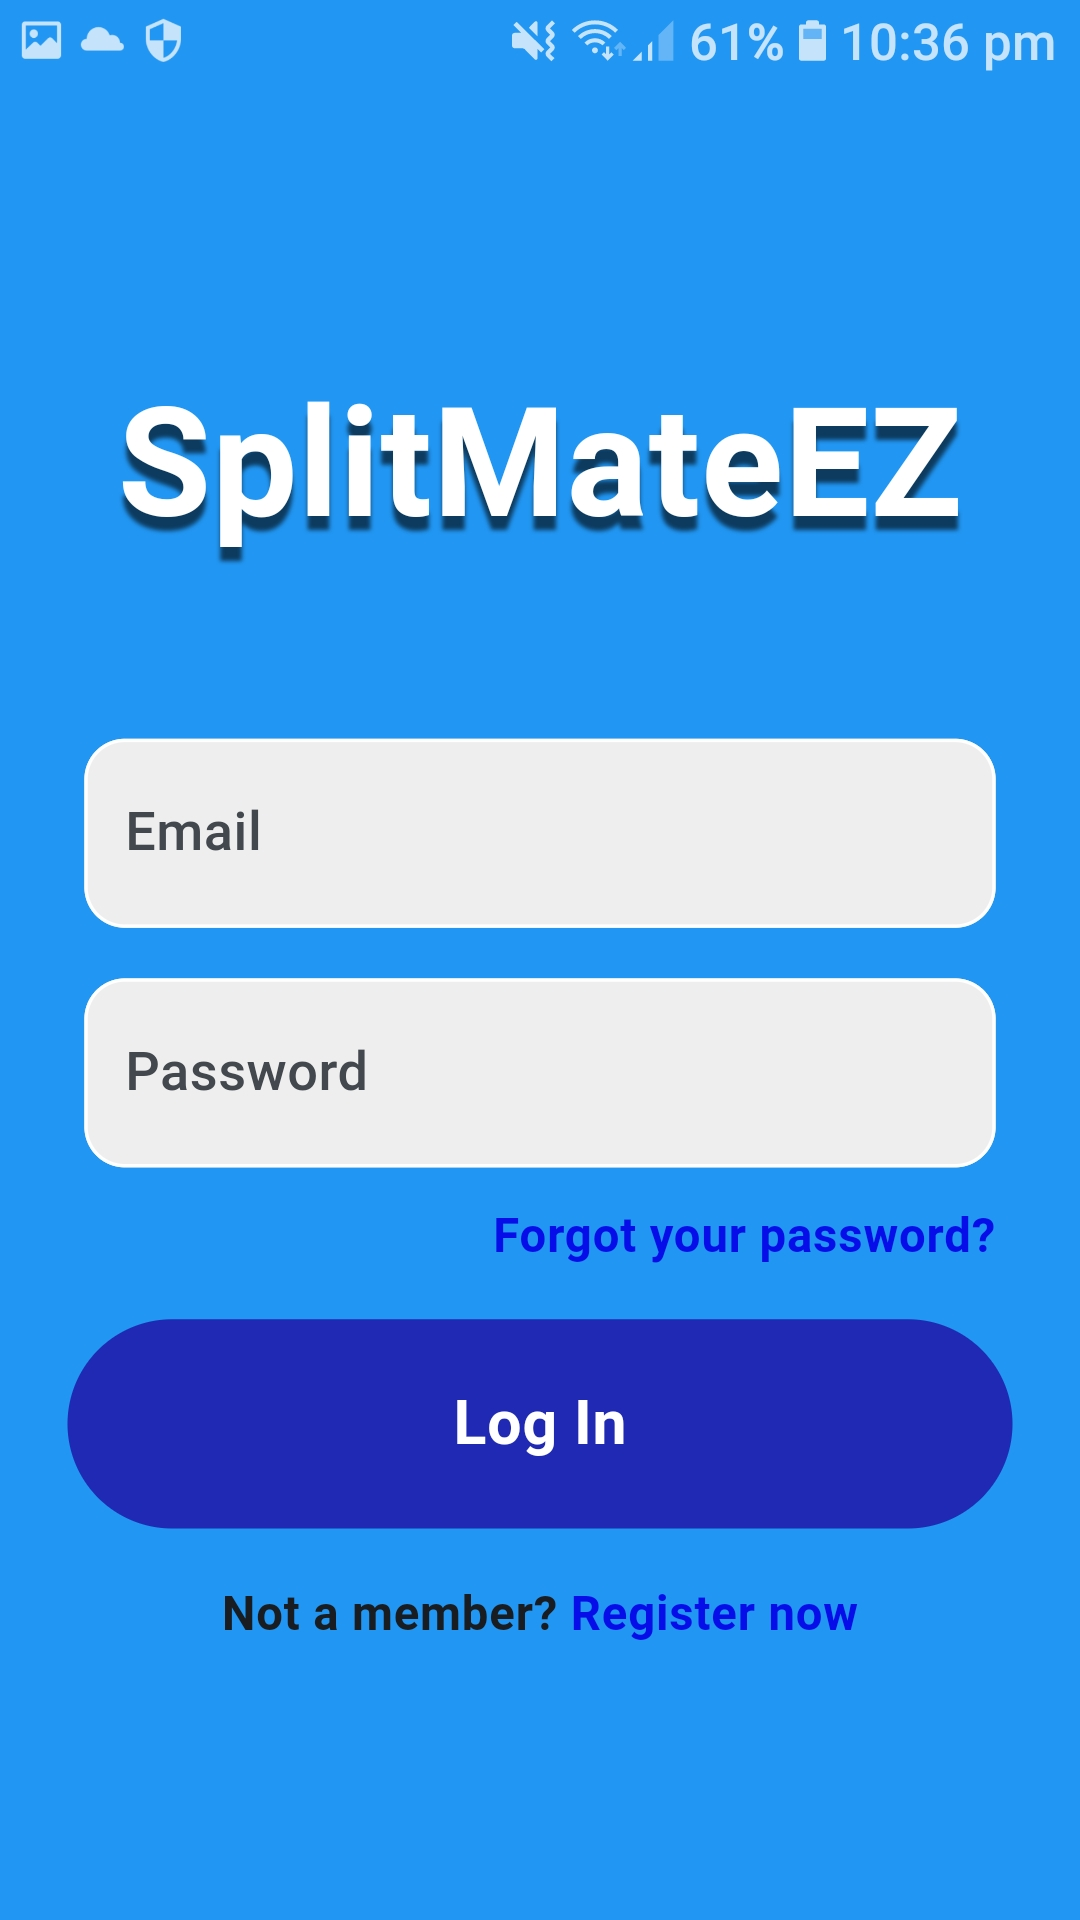
\includegraphics[width=\linewidth]{logIn.jpg}
    \caption{Log In Page}
    \label{fig:logIn}
  \end{subfigure}
  \caption{Authentication Pages}
\end{figure}

If the user forgets the password, they can reset it by clicking the "Forgot your password?" link on the login page (Figure~\ref{fig:logIn}). The application will send an email to the user's registered email address with One Time Password (OTP) to reset the password. The user can then enter the OTP and set a new password to log in to the application (Figure~\ref{fig:resetPassword}).

\begin{figure}[h]
  \centering
  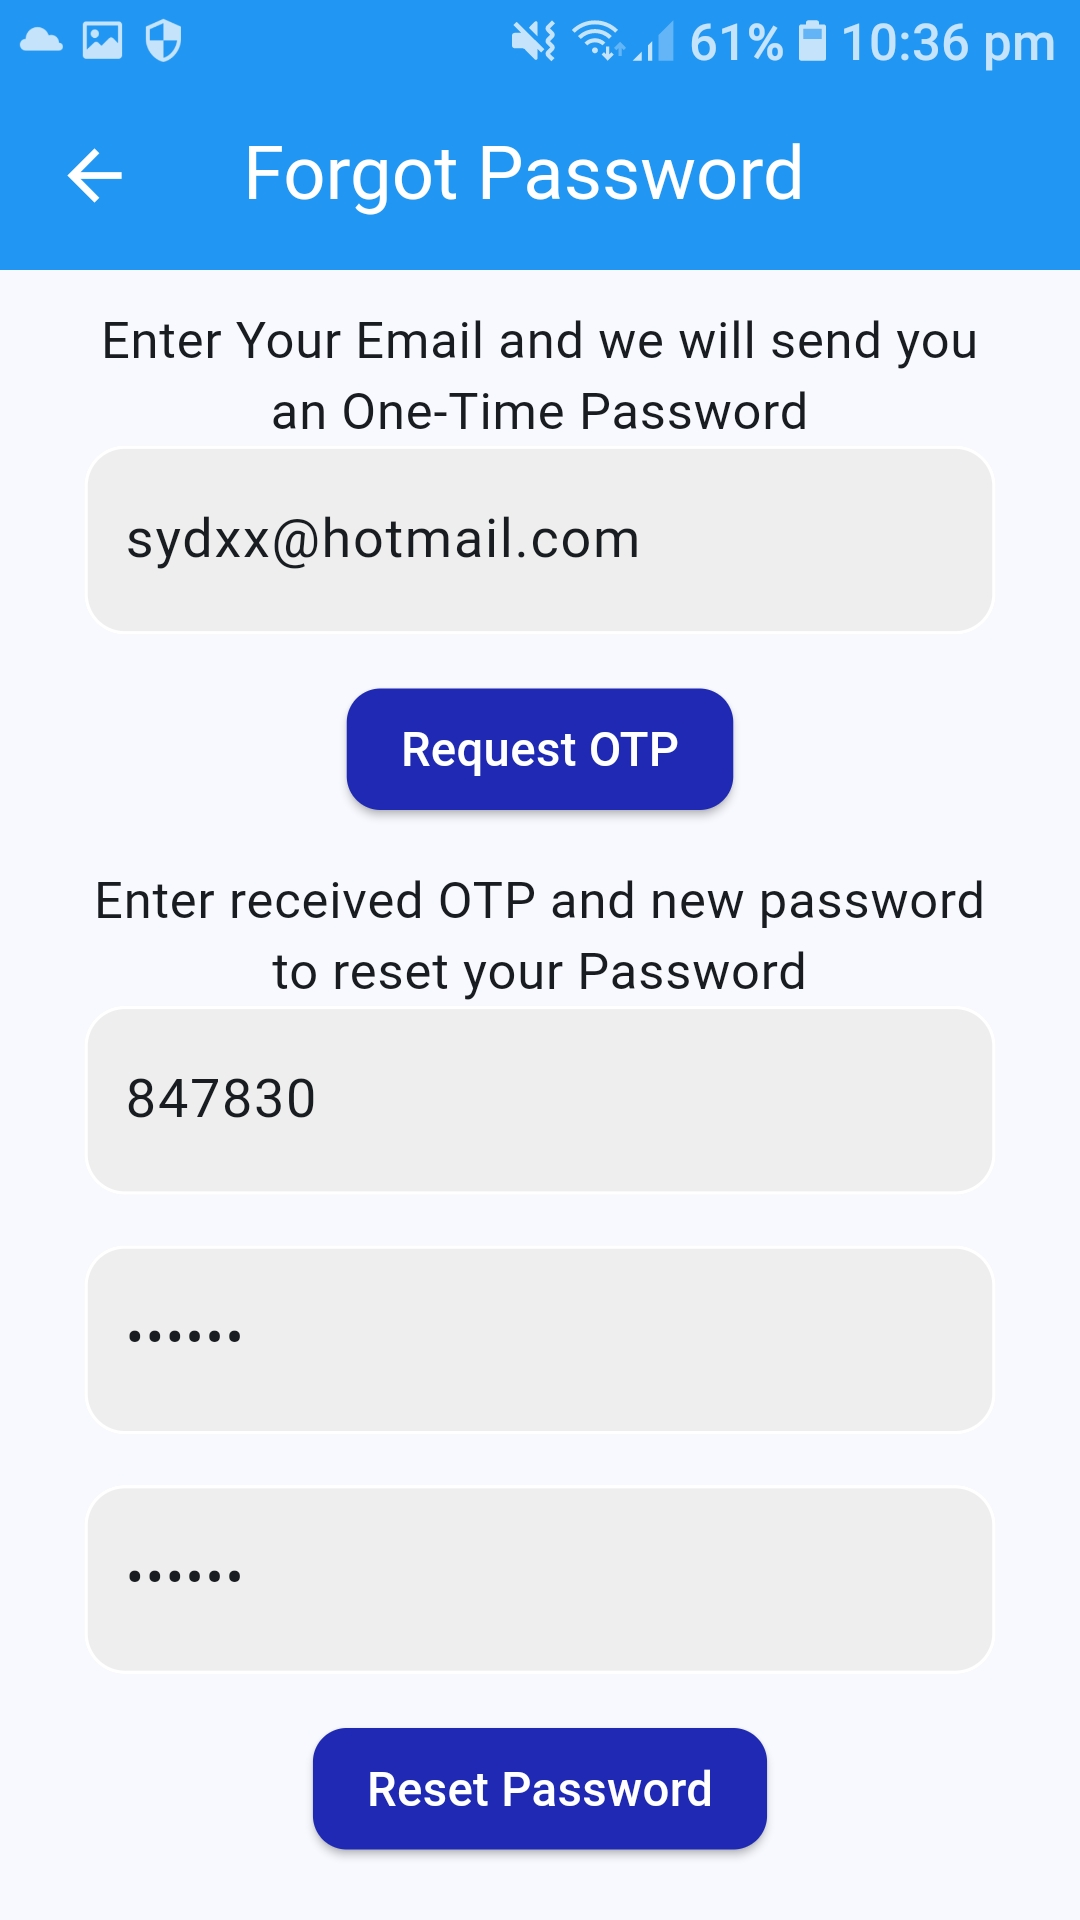
\includegraphics[width=0.24\textwidth]{resetPassword.jpg}
  \caption{Reset Password Page}
  \label{fig:resetPassword}
\end{figure}

\subsubsection{Notifications}
The notification function allows residents to receive real-time notifications about their unpaid bills or strangers trespassing (Figure~\ref{fig:warnings}). The application sends push notifications to the user's device when a new notification is generated. The user can view the notifications by clicking on the notification badge in the notification centre.

\begin{figure}[h]
  \centering
  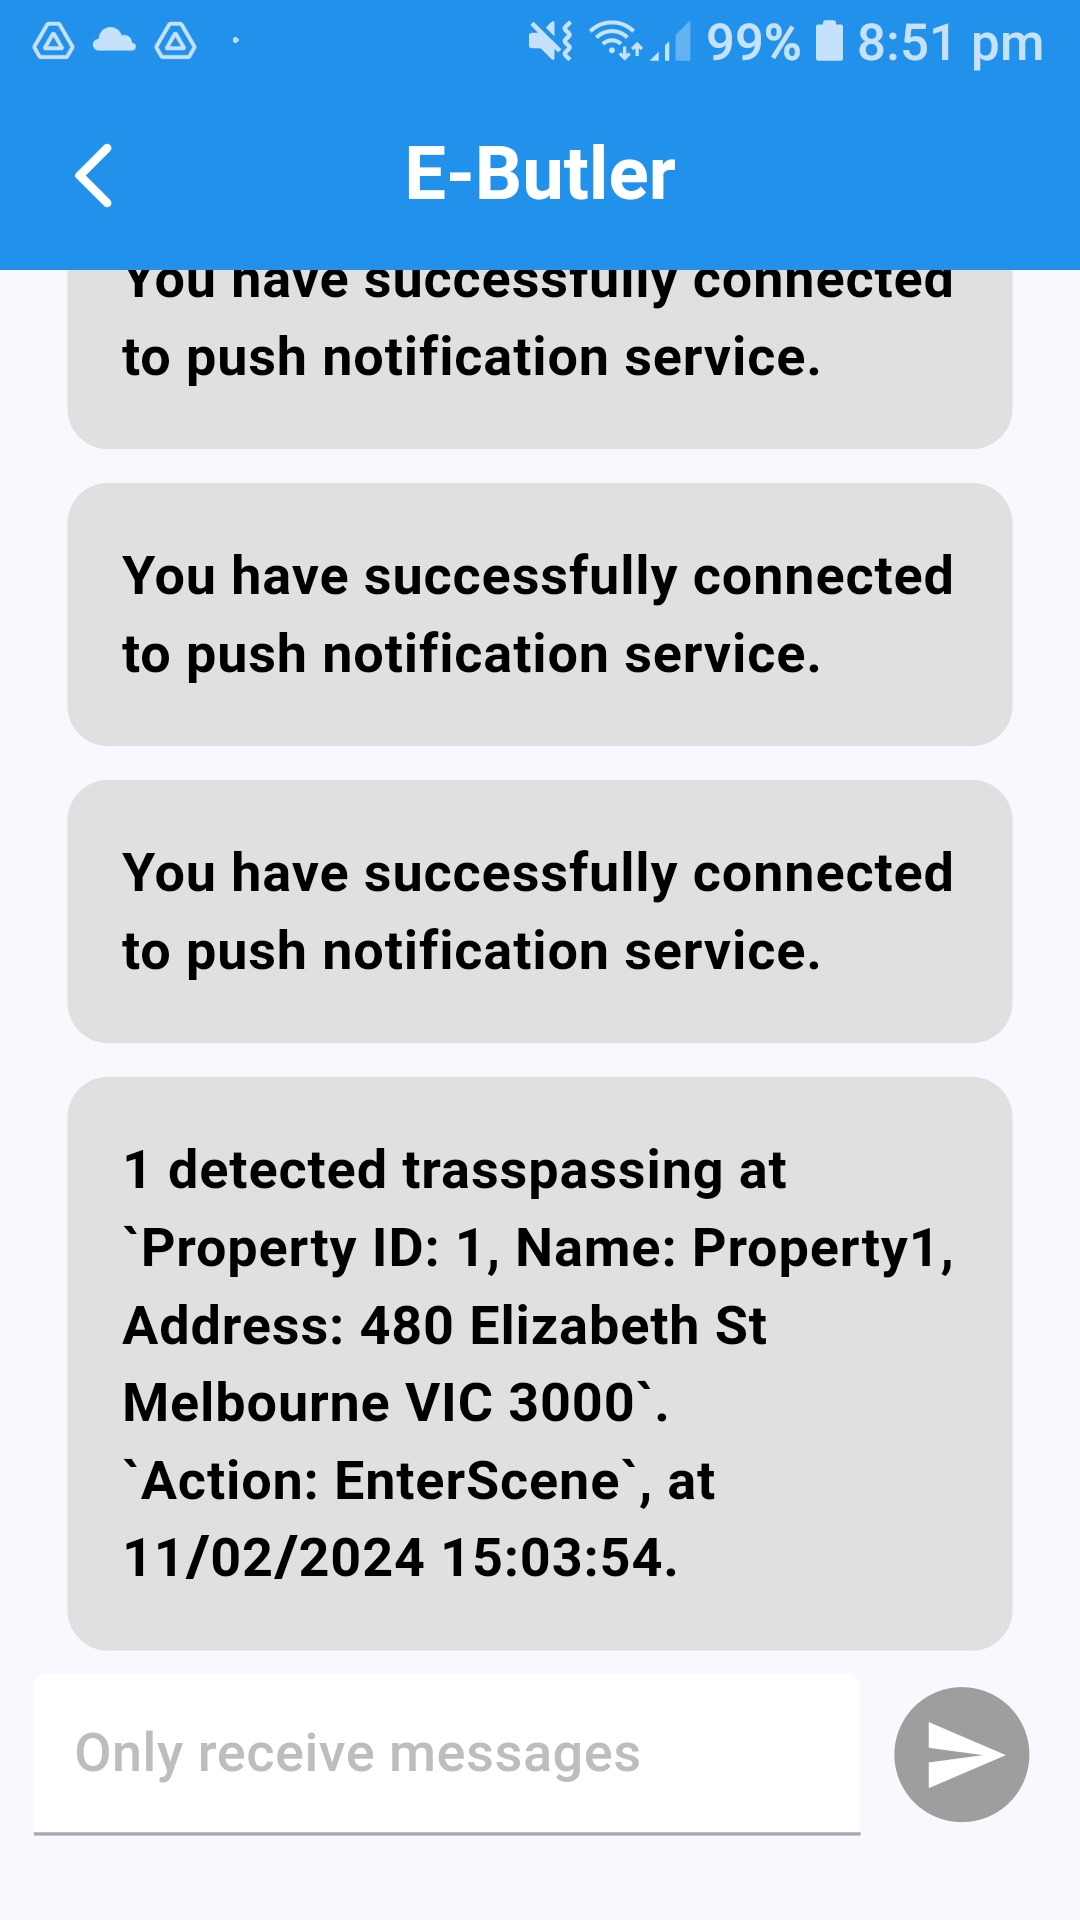
\includegraphics[width=0.24\textwidth]{onlyRecceiveWarnings.jpg}
  \caption{Received Notifications}
  \label{fig:warnings}
\end{figure}

\subsubsection{Communication}
The communication function allows residents to communicate with the landlord and landlord can communicate with all residents (Figure~\ref{fig:chatList}). Residents can send messages to the landlord to report any issues or ask questions. The landlord can send messages to all residents to inform them about any important updates or announcements (Figure~\ref{fig:chatRoom}). The chat feature provides a convenient way for residents and landlords to communicate and resolve any issues that may arise.

\begin{figure}[h]
  \centering
  \begin{subfigure}{0.24\textwidth}
    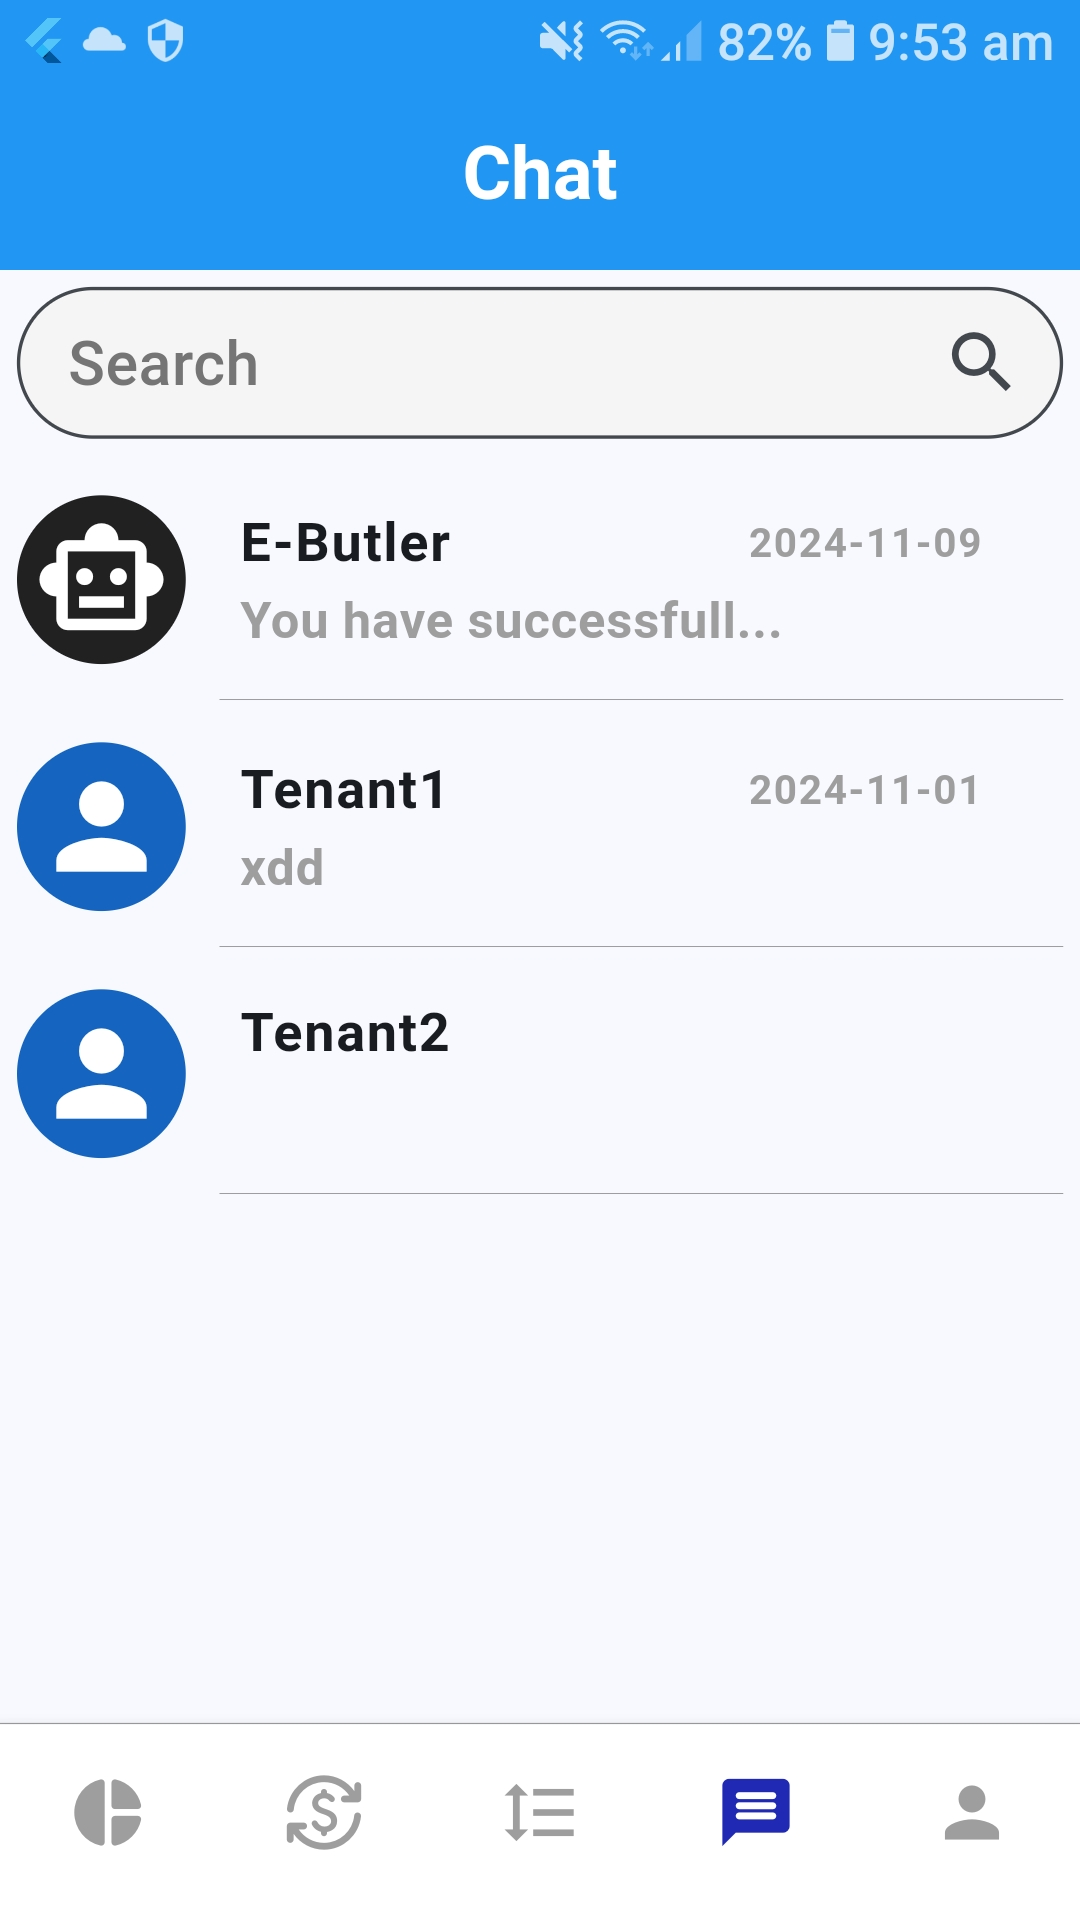
\includegraphics[width=\textwidth]{chatList.jpg}
    \caption{Chat List}
    \label{fig:chatList}
  \end{subfigure}
  \begin{subfigure}{0.24\textwidth}
    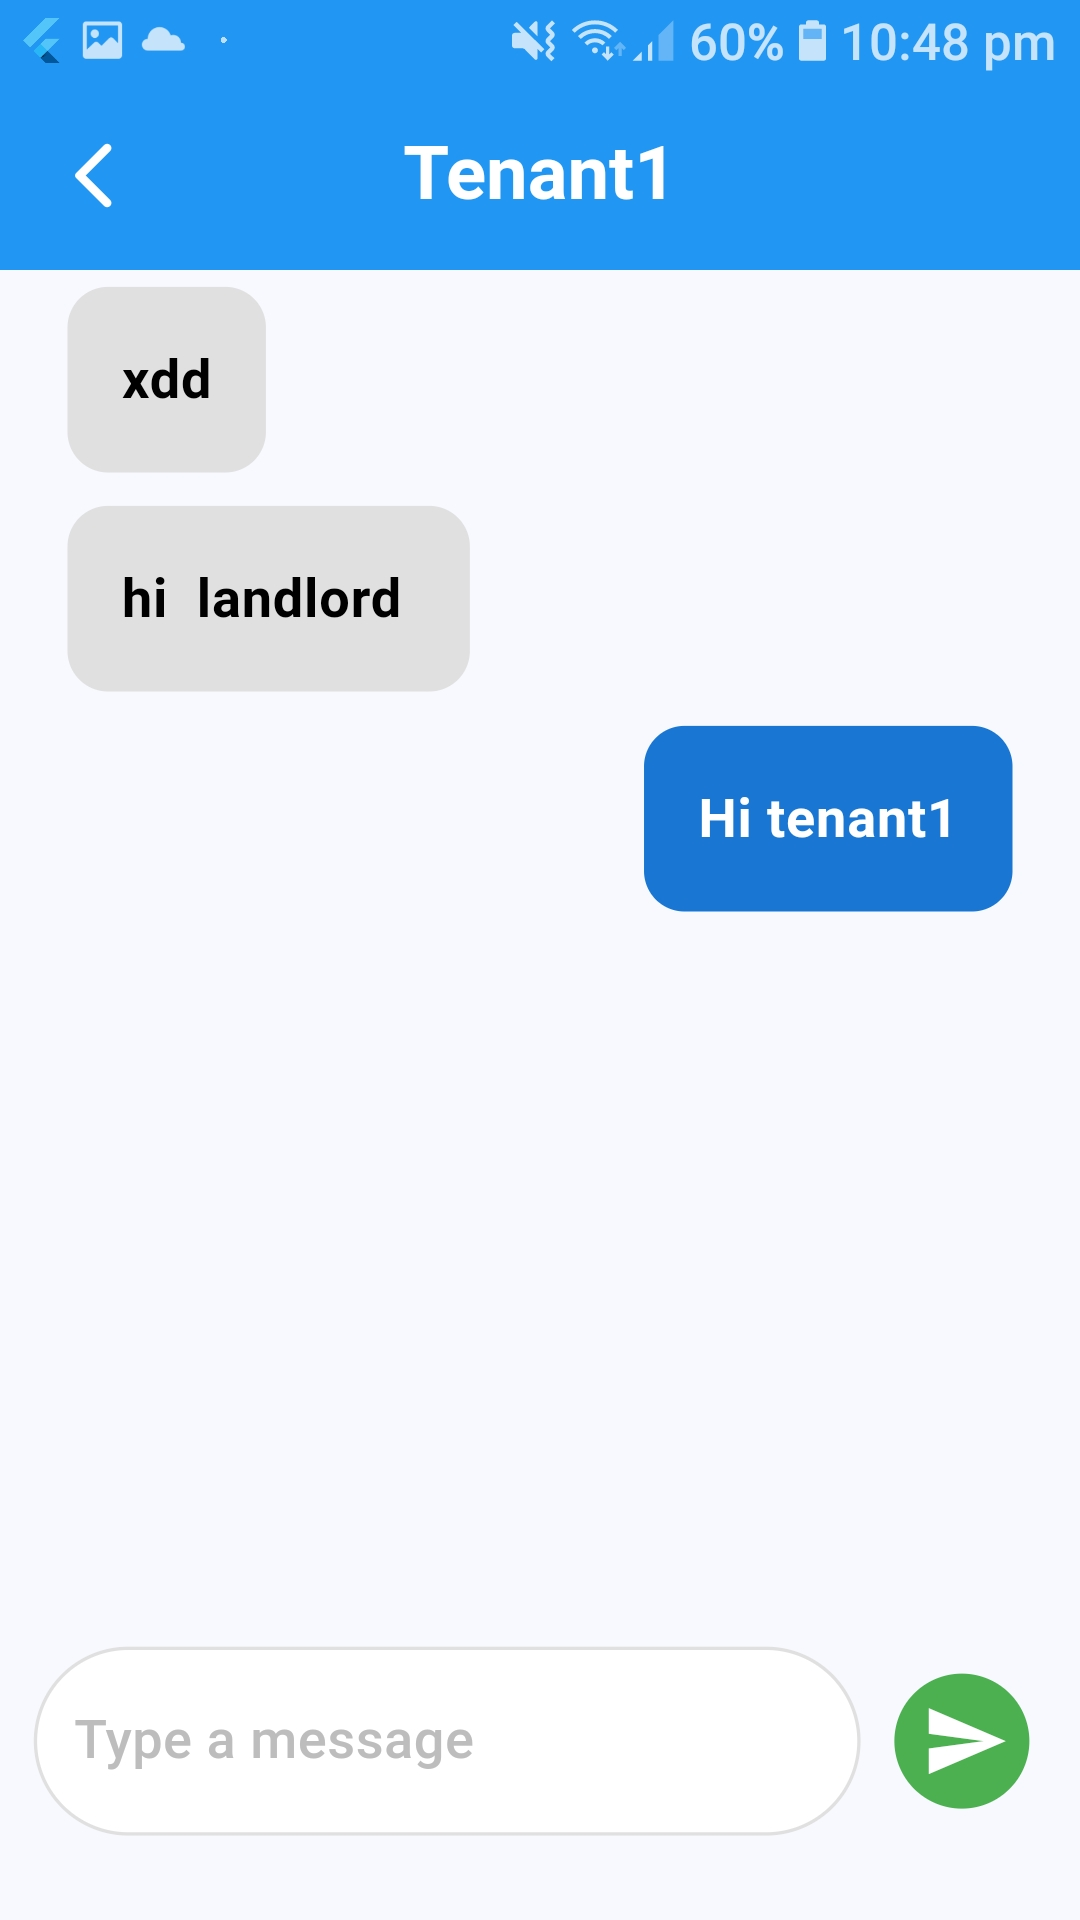
\includegraphics[width=\textwidth]{chatting.jpg}
    \caption{Chatting Page}
    \label{fig:chatRoom}
  \end{subfigure}
  \caption{Communication Pages}
\end{figure}

\subsubsection{Management}
The management function allows the landlord to add new properties and add new tenants into a property. The landlord can create a new property by entering the property details, such as the property name, address, and postcode (Figure~\ref{fig:addNewProperty}). The landlord can then add new tenants to the property by entering the tenant's email (Figure~\ref{fig:addTenant}). The landlord can also view the list of properties (Figure~\ref{fig:propertyInfo}) and tenants (Figure~\ref{fig:propertyTenants}) and edit or delete them (Figure~\ref{fig:banTenant}) as needed.

\begin{figure}[h]
  \centering
  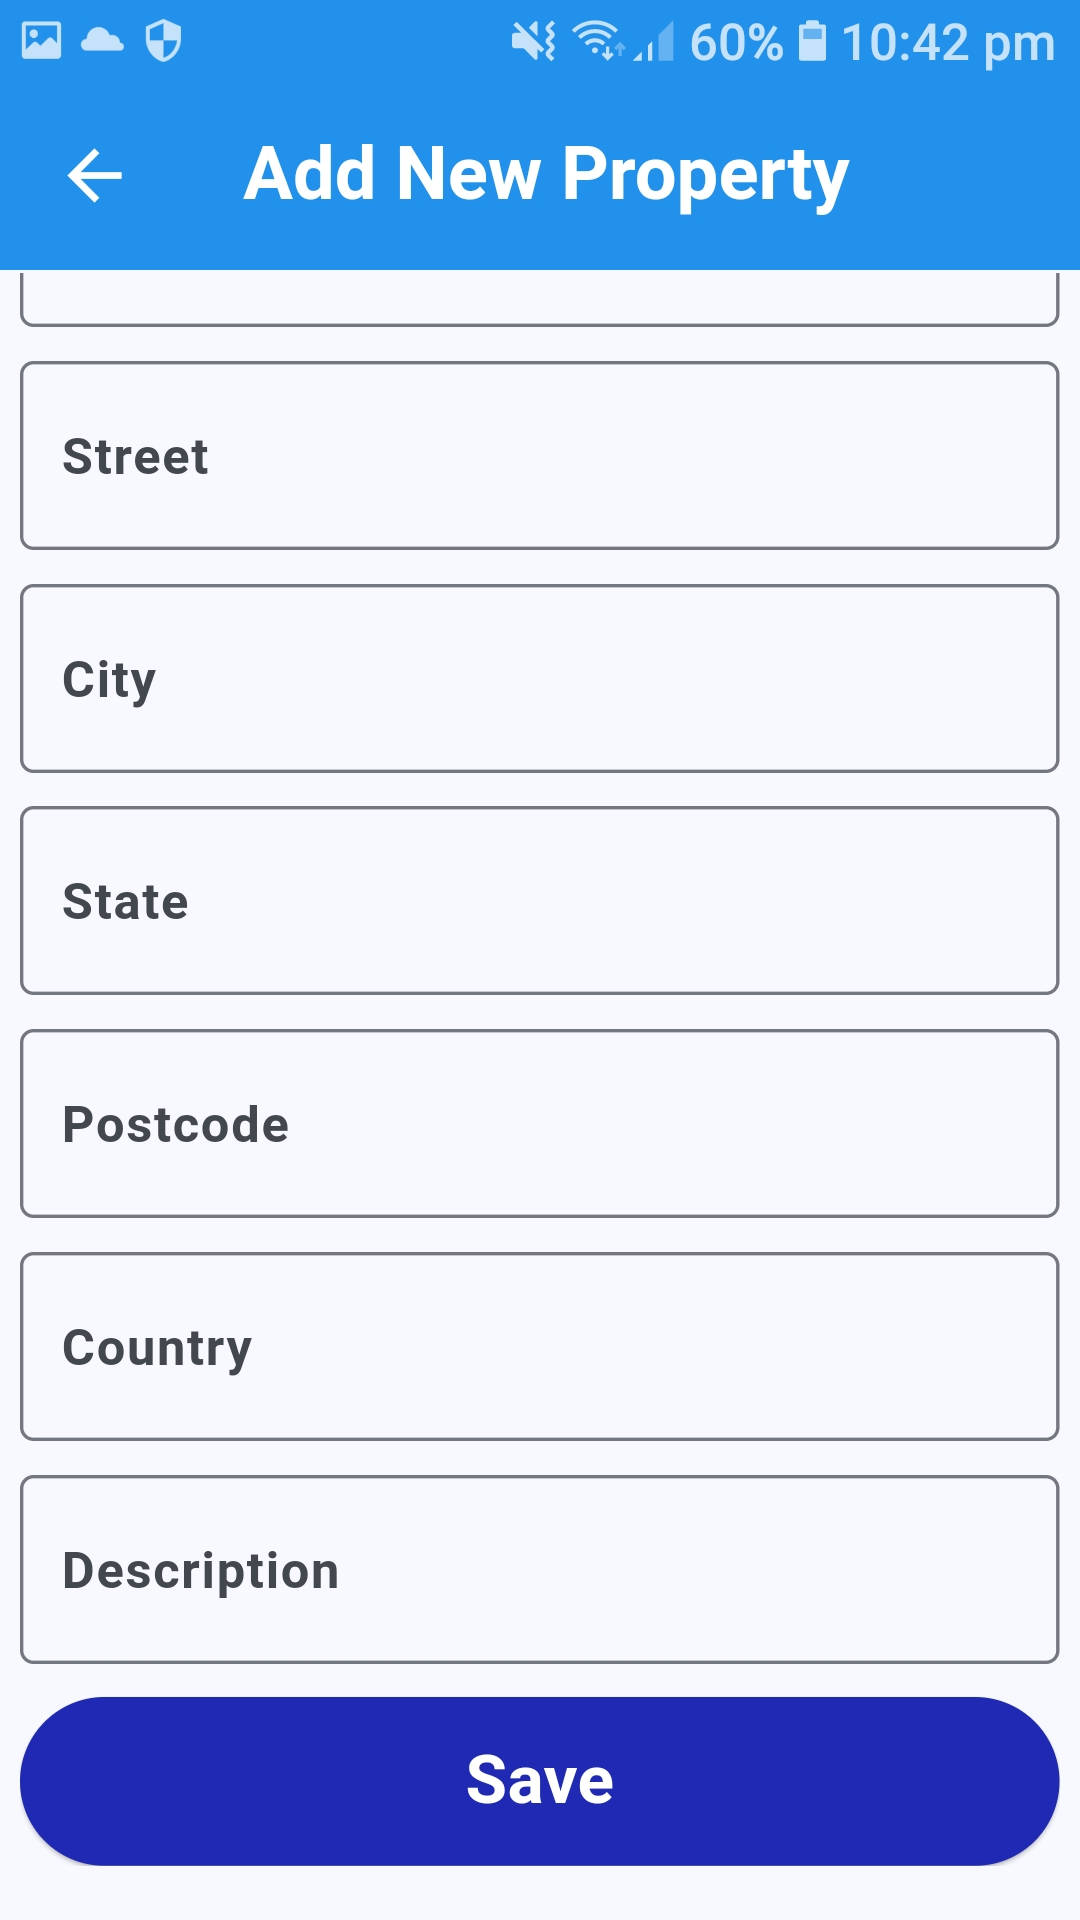
\includegraphics[width=0.24\textwidth]{addNewProperty.jpg}
  \caption{Add new property}
  \label{fig:addNewProperty}
\end{figure}

\begin{figure}[h]
  \centering
  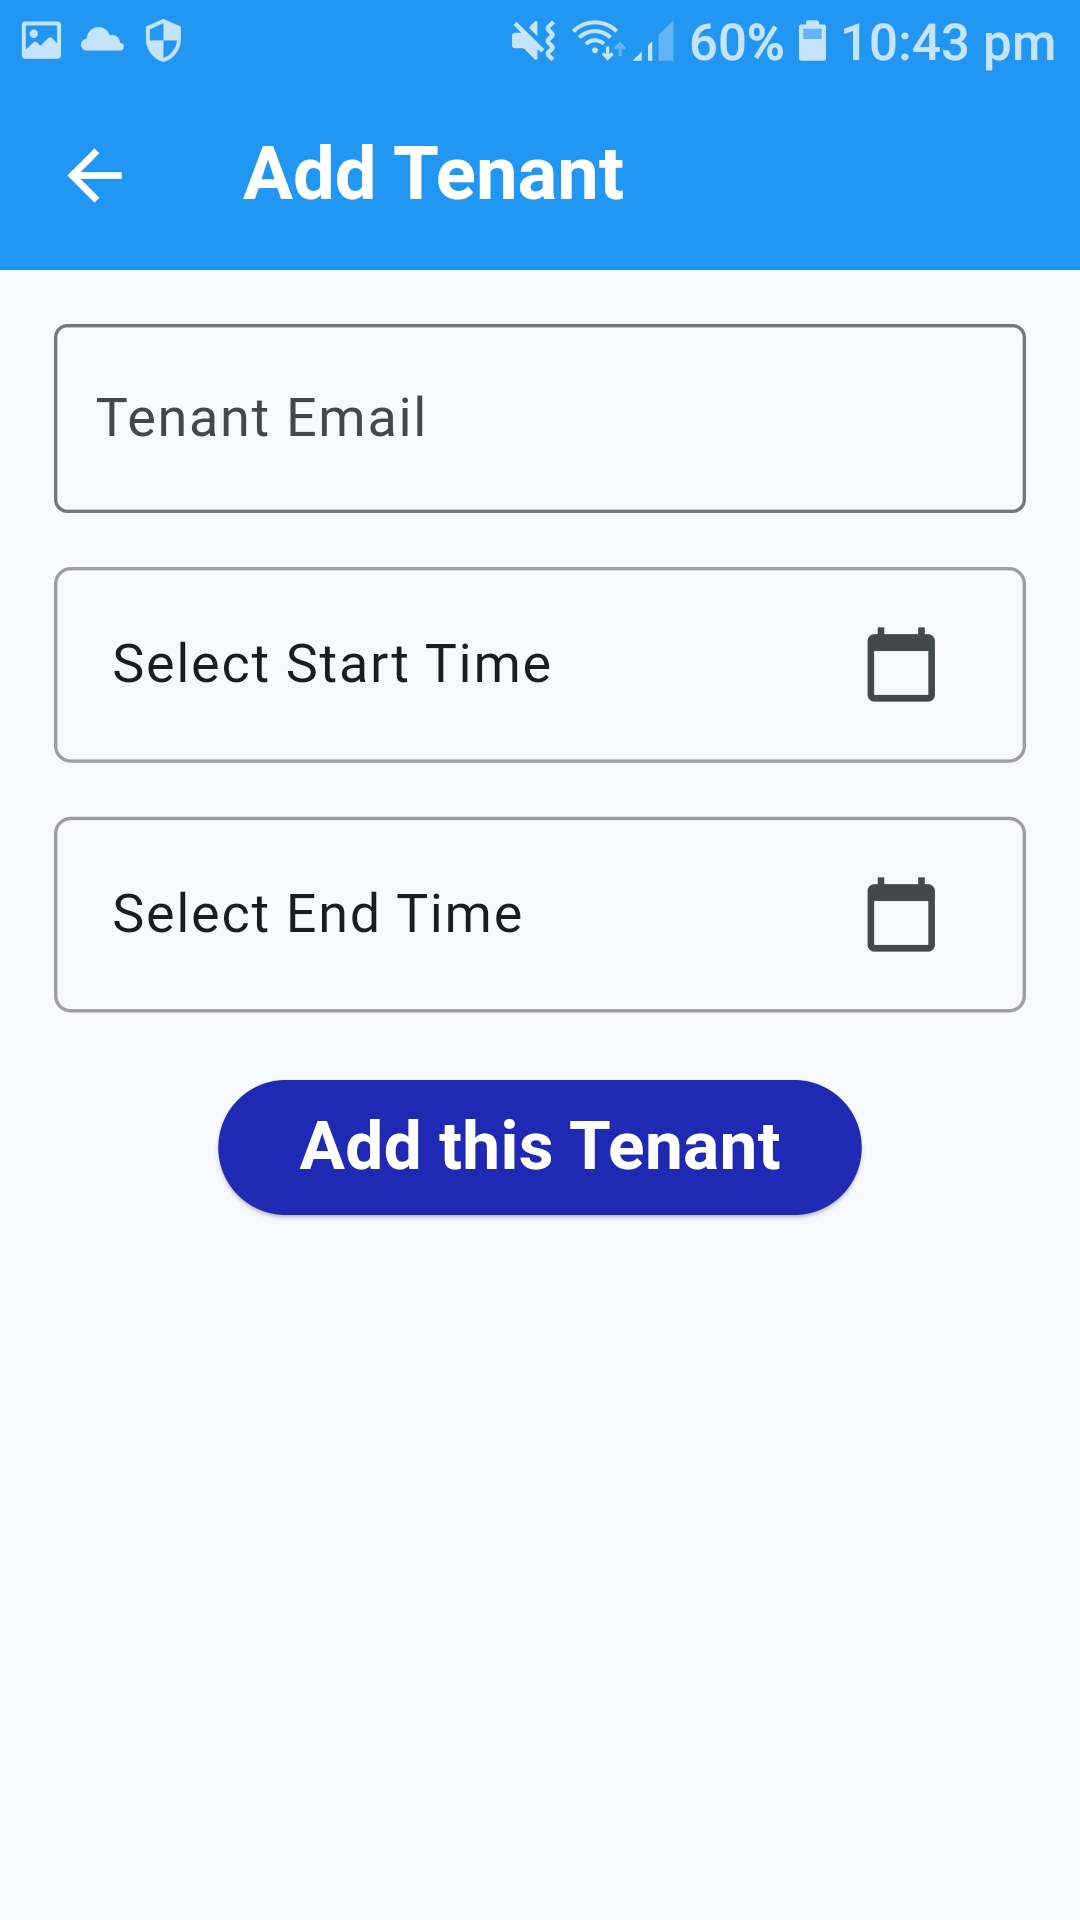
\includegraphics[width=0.24\textwidth]{addTenant.jpg}
  \caption{Add new tenant}
  \label{fig:addTenant}
\end{figure}

\begin{figure}[h]
  \centering
  \begin{subfigure}{0.24\textwidth}
    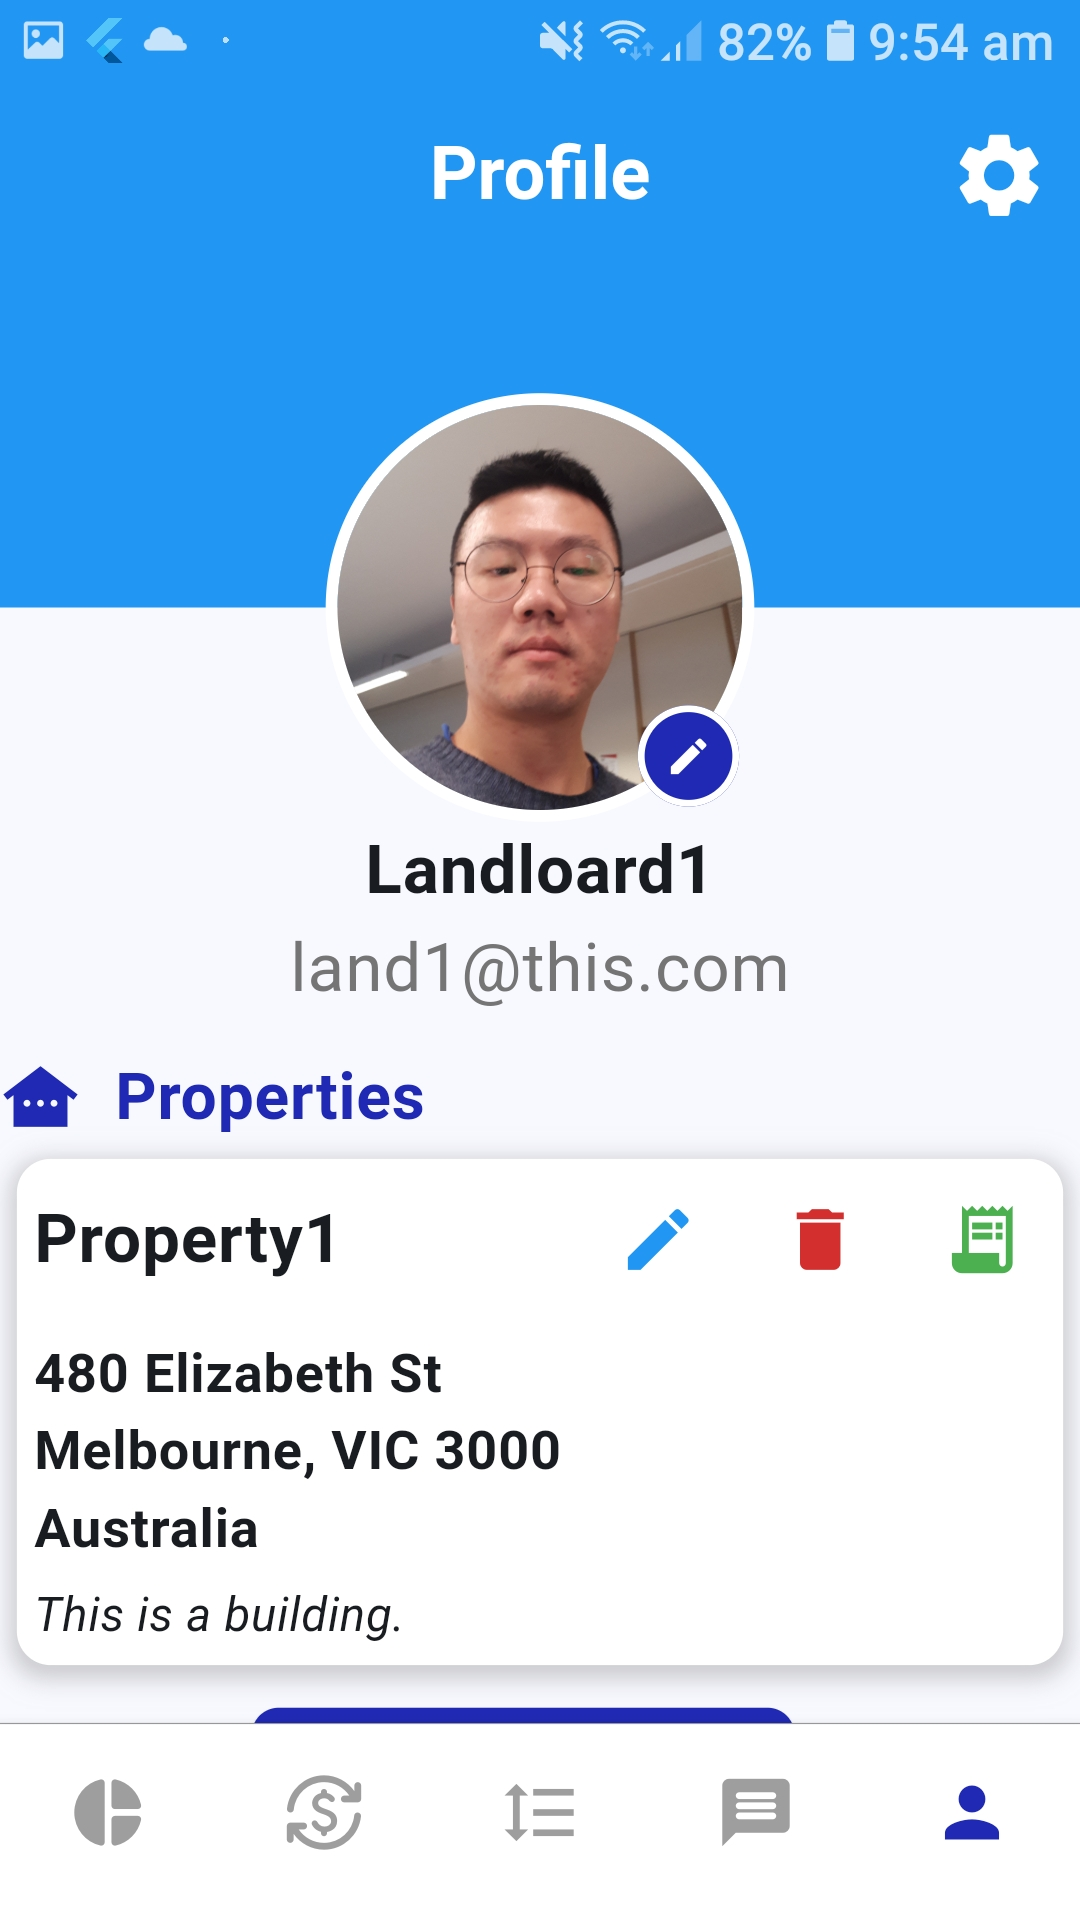
\includegraphics[width=\textwidth]{propertyInfo.jpg}
    \caption{View property info}
    \label{fig:propertyInfo}
  \end{subfigure}
  \begin{subfigure}{0.24\textwidth}
    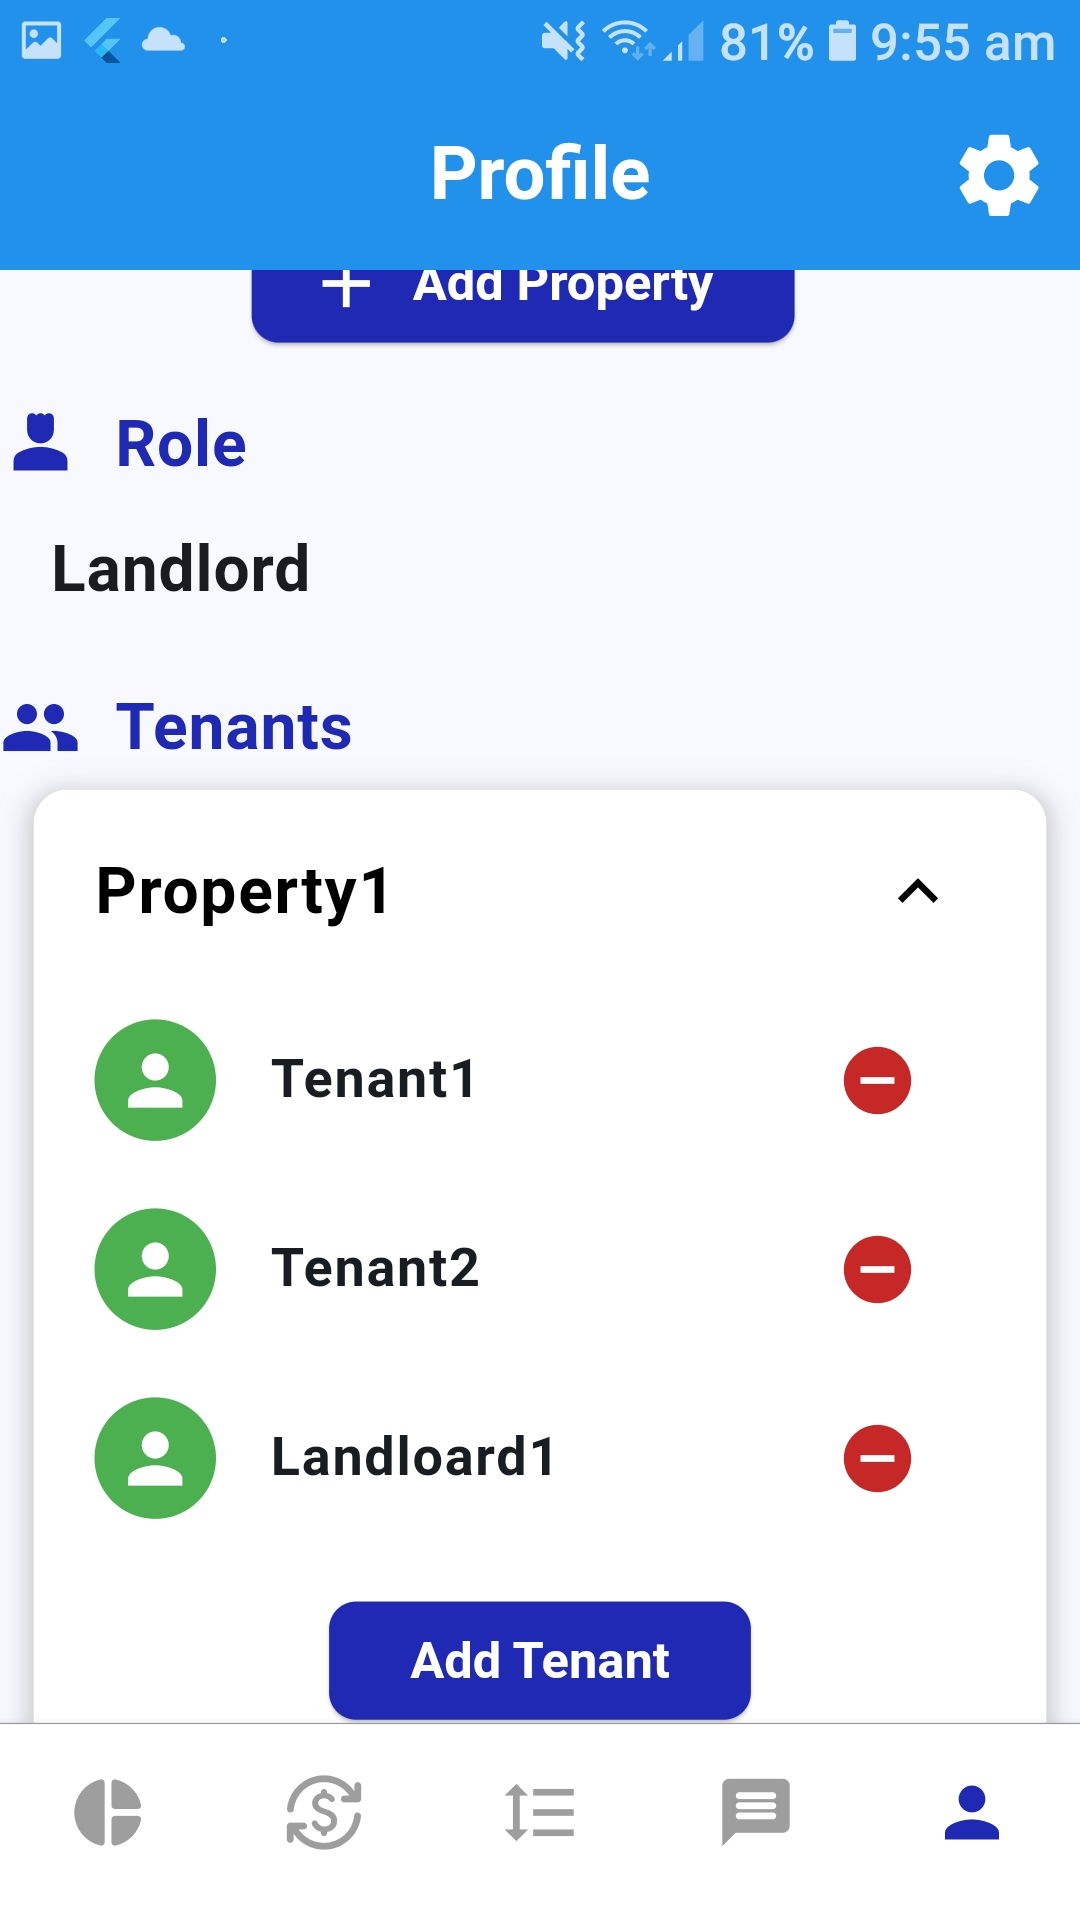
\includegraphics[width=\textwidth]{propertyTenants.jpg}
    \caption{Tenants of a property}
    \label{fig:propertyTenants}
  \end{subfigure}
  \caption{House Management Pages}
\end{figure}

\begin{figure}[h]
  \centering
  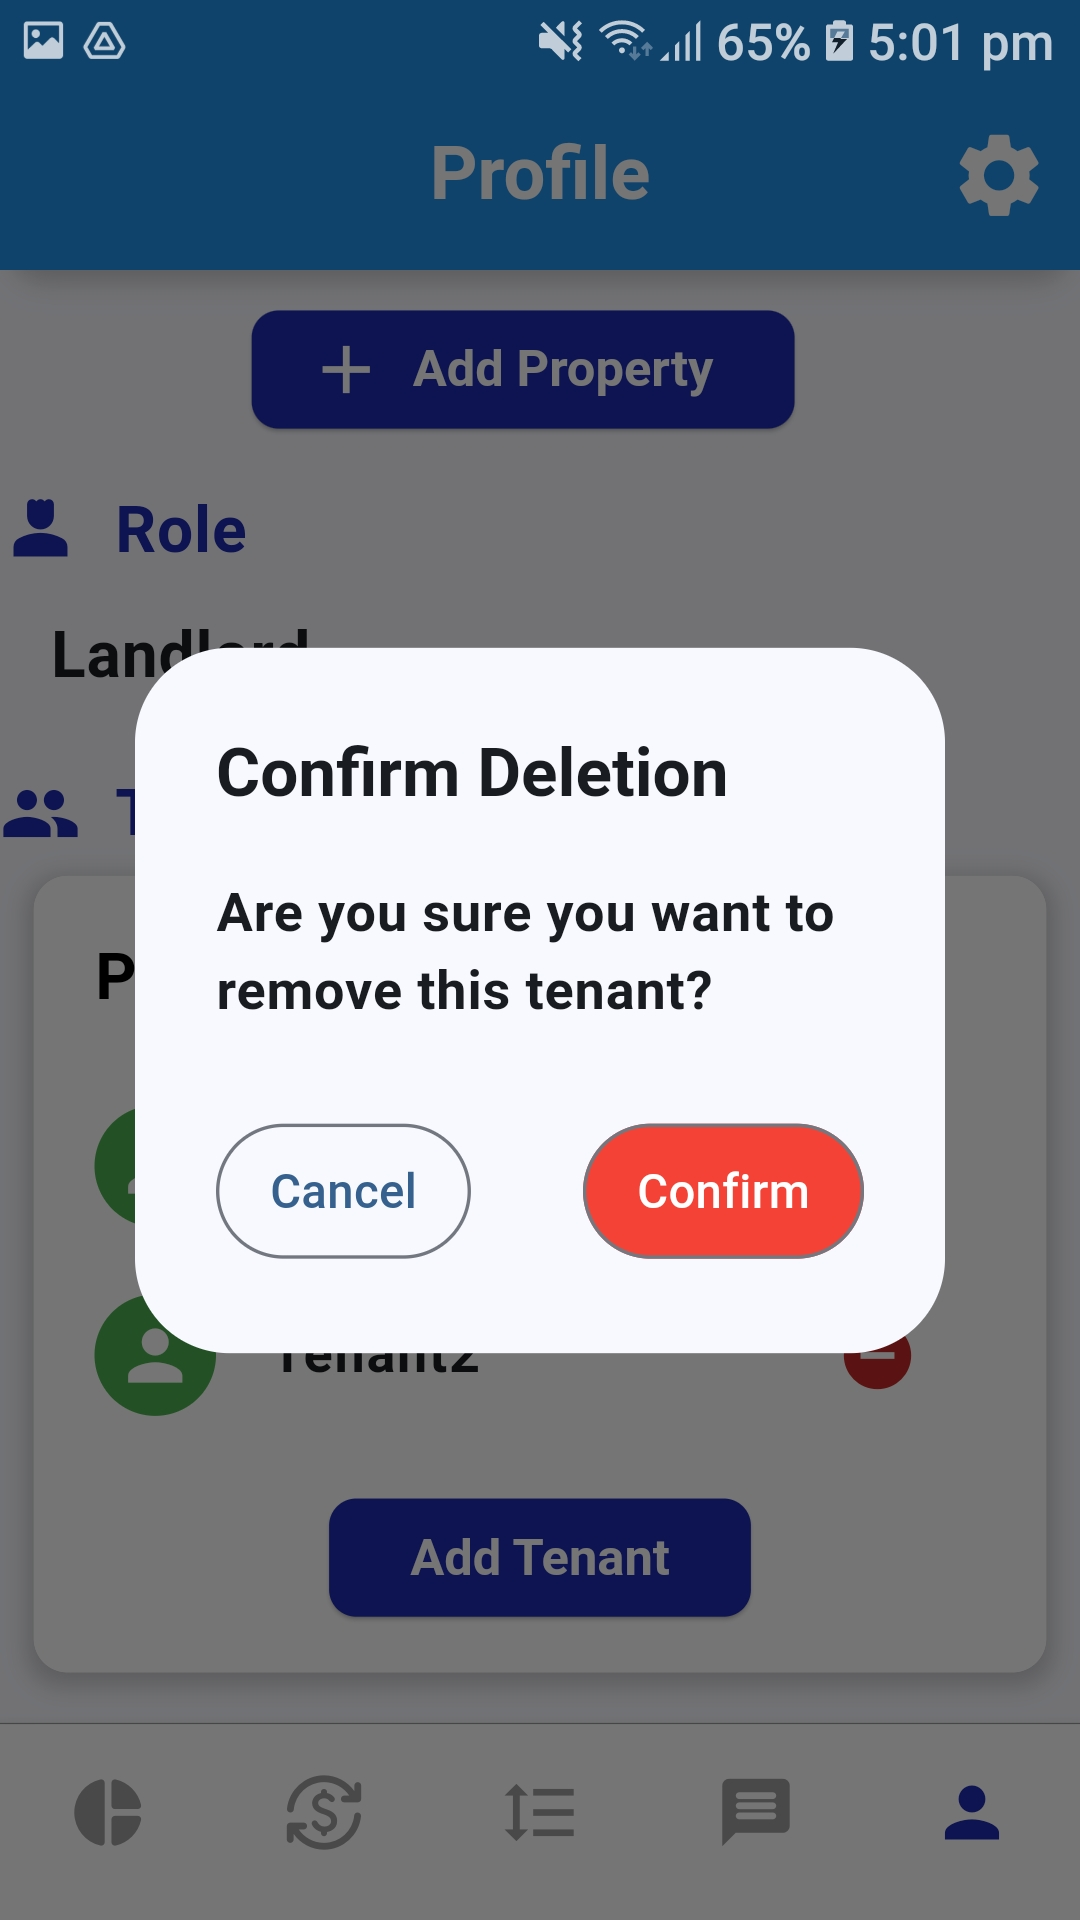
\includegraphics[width=0.24\textwidth]{banTenant.jpg}
  \caption{Ban a tenant}
  \label{fig:banTenant}
\end{figure}

% ===============================================================
\subsection{Specialized Functions}
Some specialized functions have been implemented in our application to provide additional features and enhance the user experience. These functions include face recognition, text recognition, usage tracking through graphs, actions history through timeline, pay bills, and generate report using Large Language Model.

\subsubsection{Face Recognition}
A new registered user cannot access other pages until they upload their profile photo by taking a photo through the phone camera (Figure~\ref{fig:RequireProfilePhoto}).
The face recognition function allows residents to upload their profile photo only through the phone camera and ensures there is a face in that photo (Figure~\ref{fig:faceDetecting}) using \specialterm{Google's ML Kit Face Detection} SDK. If the photo does not contain a face, the user will not have access to other pages and must retake a proper photo (Figure~\ref{fig:noFace}). If a face is successfully detected, it will be immediately uploaded to the server (Figure~\ref{fig:faceCheckSuccess}).
This feature provides an additional layer of security and ensures that only authorized, real users can access the application.

\begin{figure}[h]
  \centering
  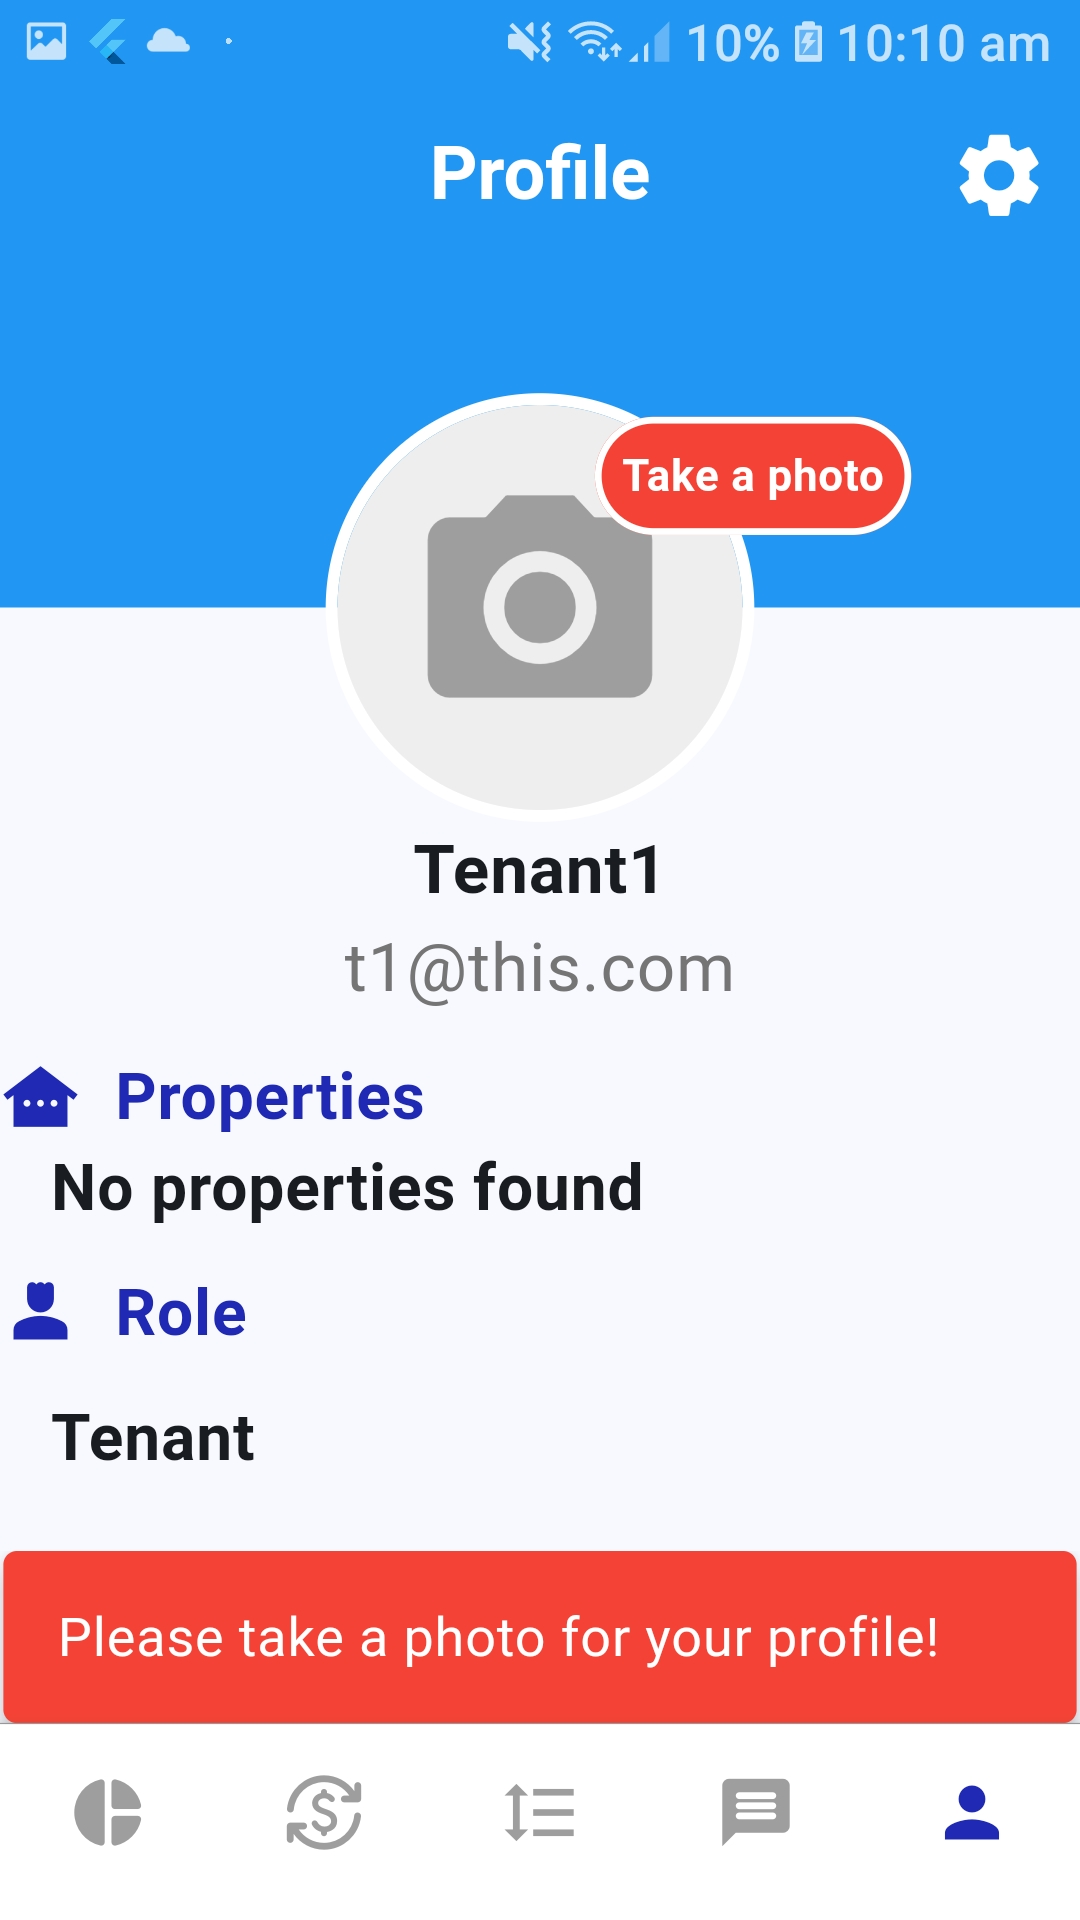
\includegraphics[width=0.24\textwidth]{RequireProfilePhoto.jpg}
  \caption{Profile Photo Required}
  \label{fig:RequireProfilePhoto}
\end{figure}
\begin{figure}[h]
  \centering
  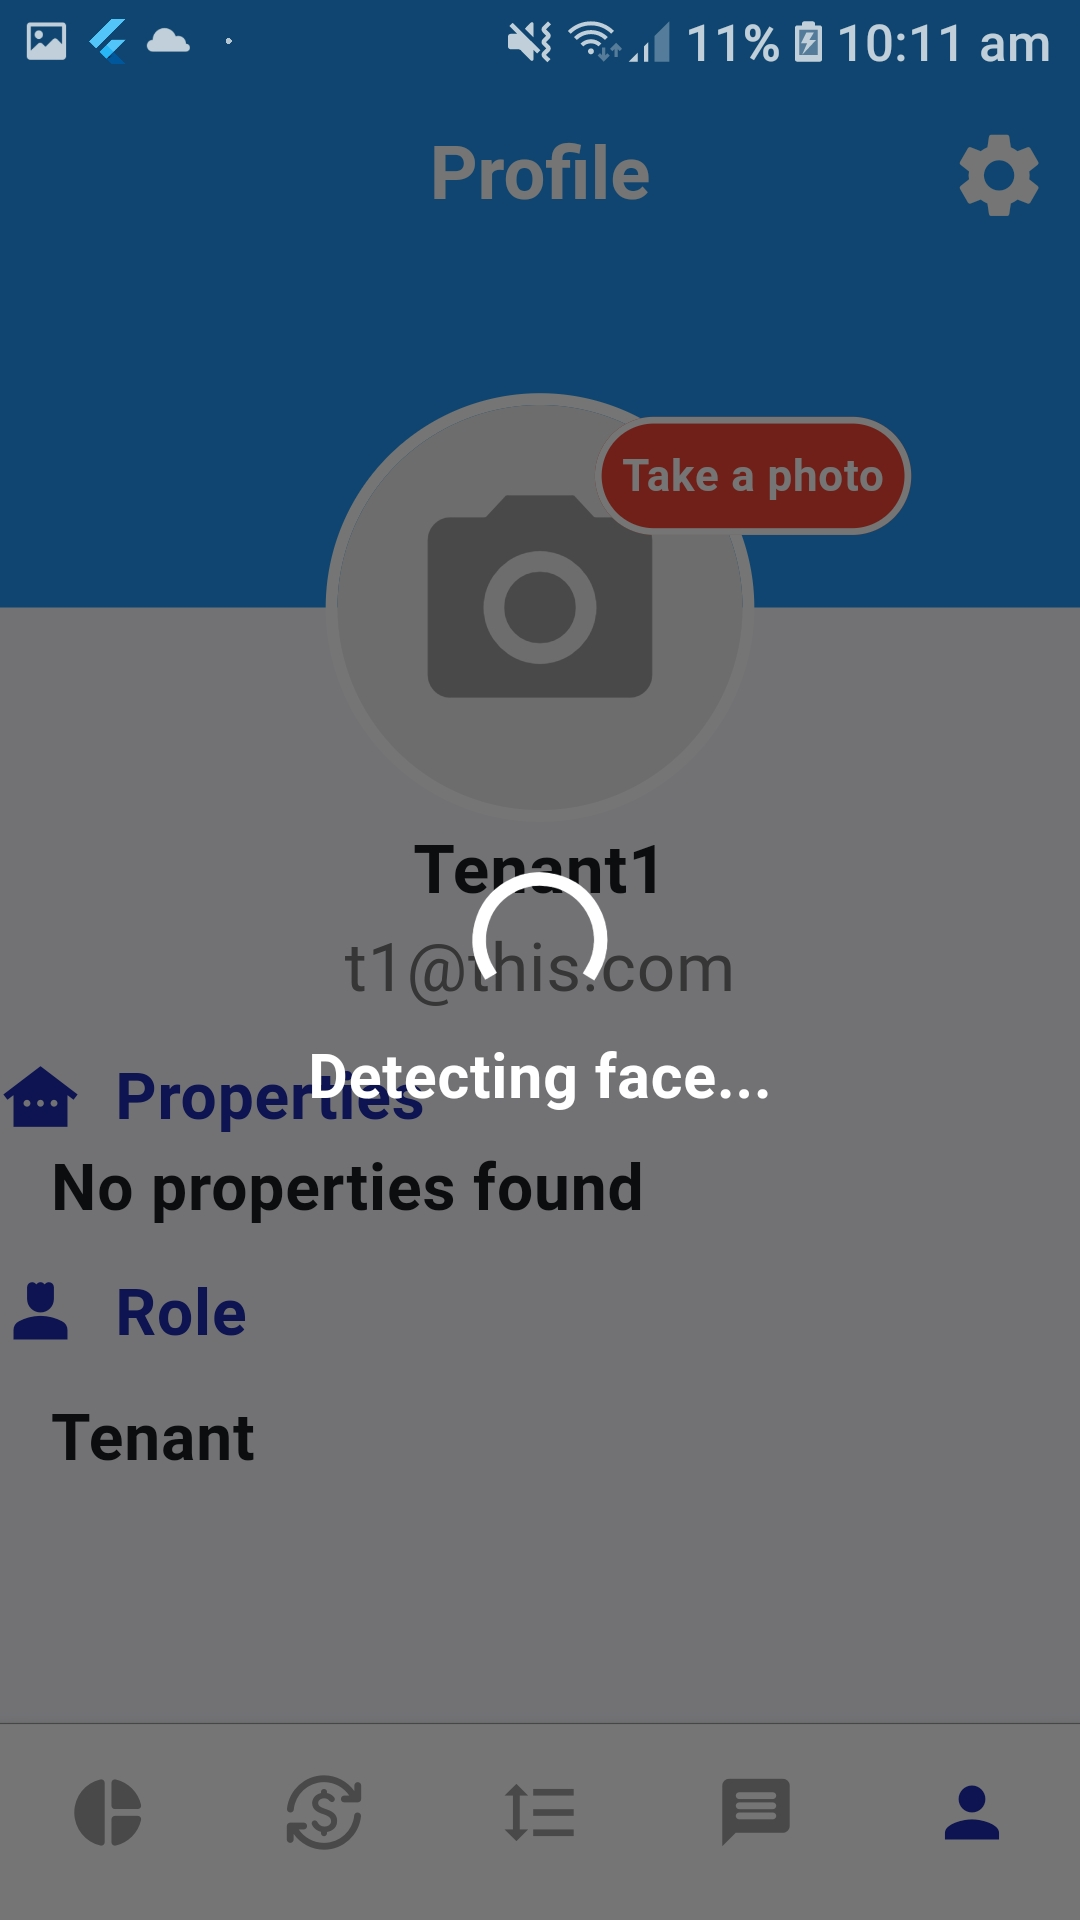
\includegraphics[width=0.24\textwidth]{faceDetecting.jpg}
  \caption{Face Detecting}
  \label{fig:faceDetecting}
\end{figure}
\begin{figure}[h]
  \centering
  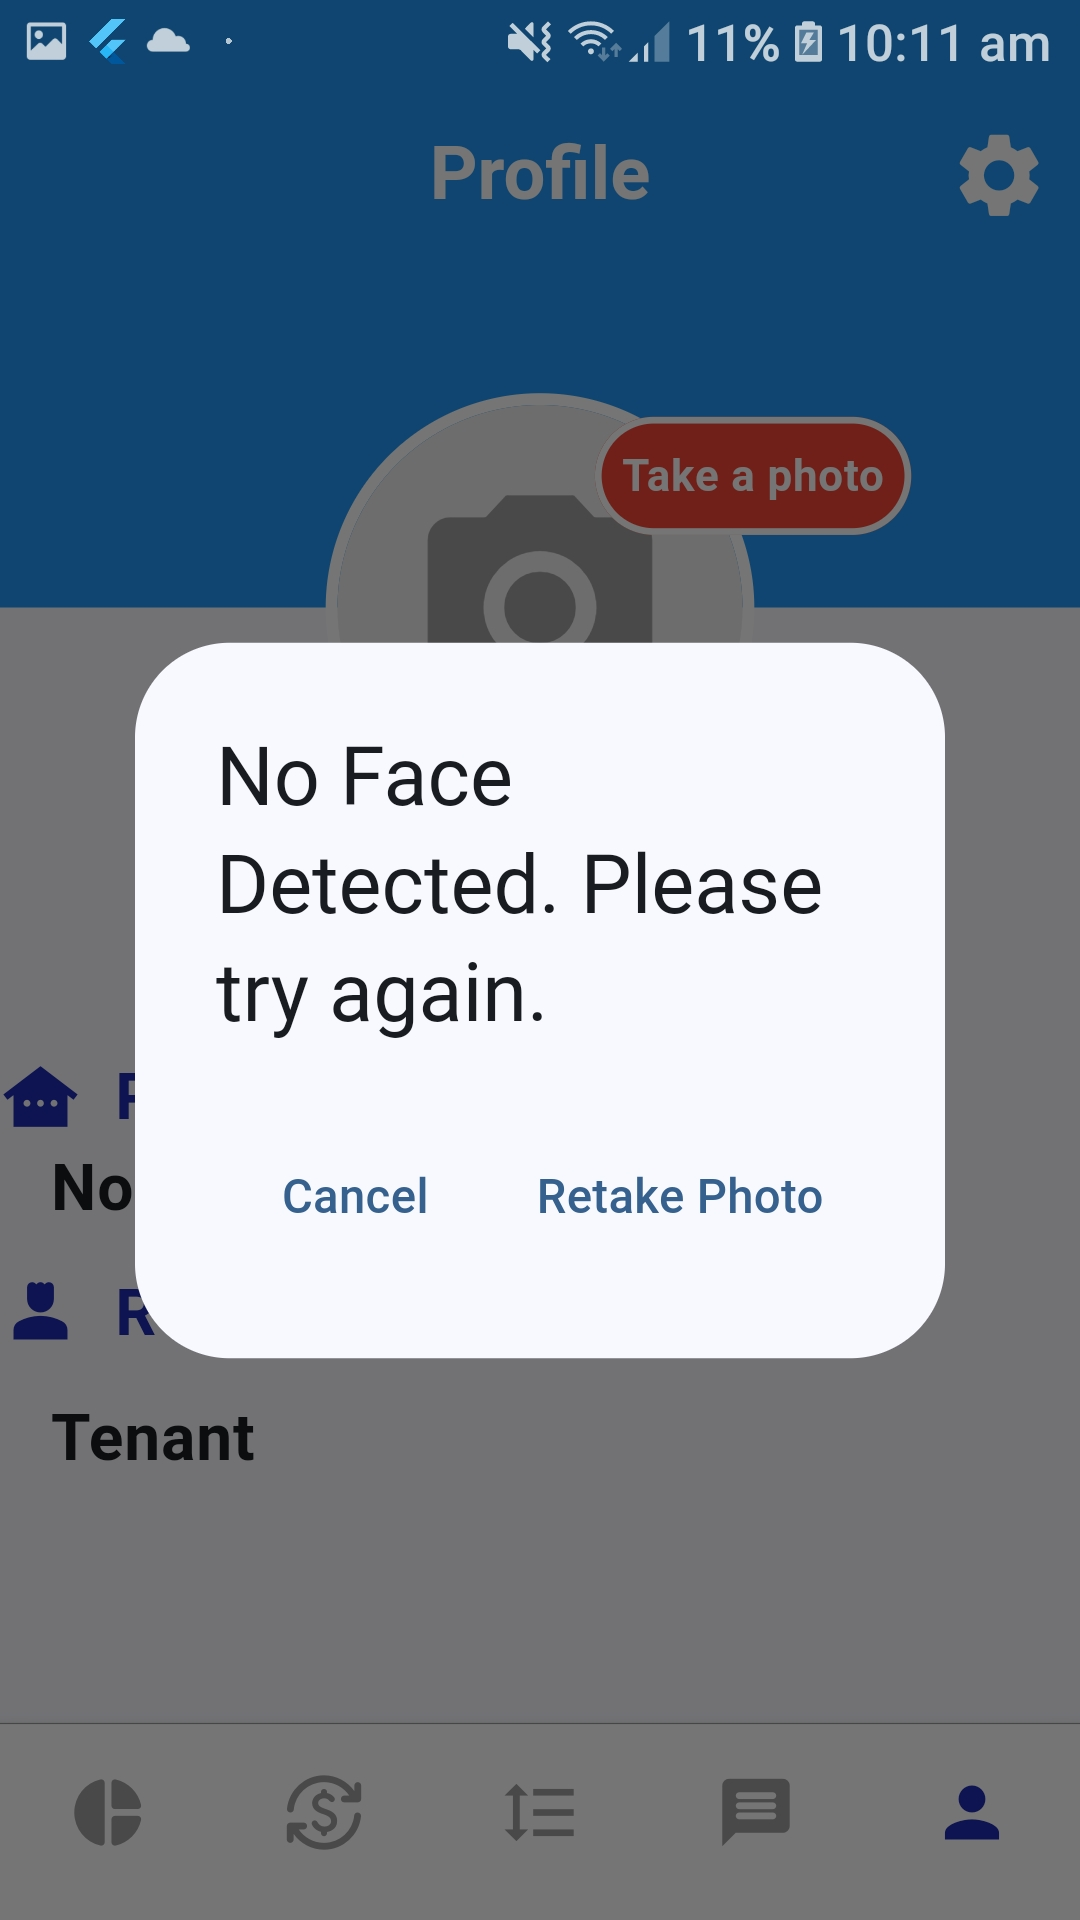
\includegraphics[width=0.24\textwidth]{faceCheckFailed.jpg}
  \caption{Face Not Detected}
  \label{fig:noFace}
\end{figure}
\begin{figure}[h]
  \centering
  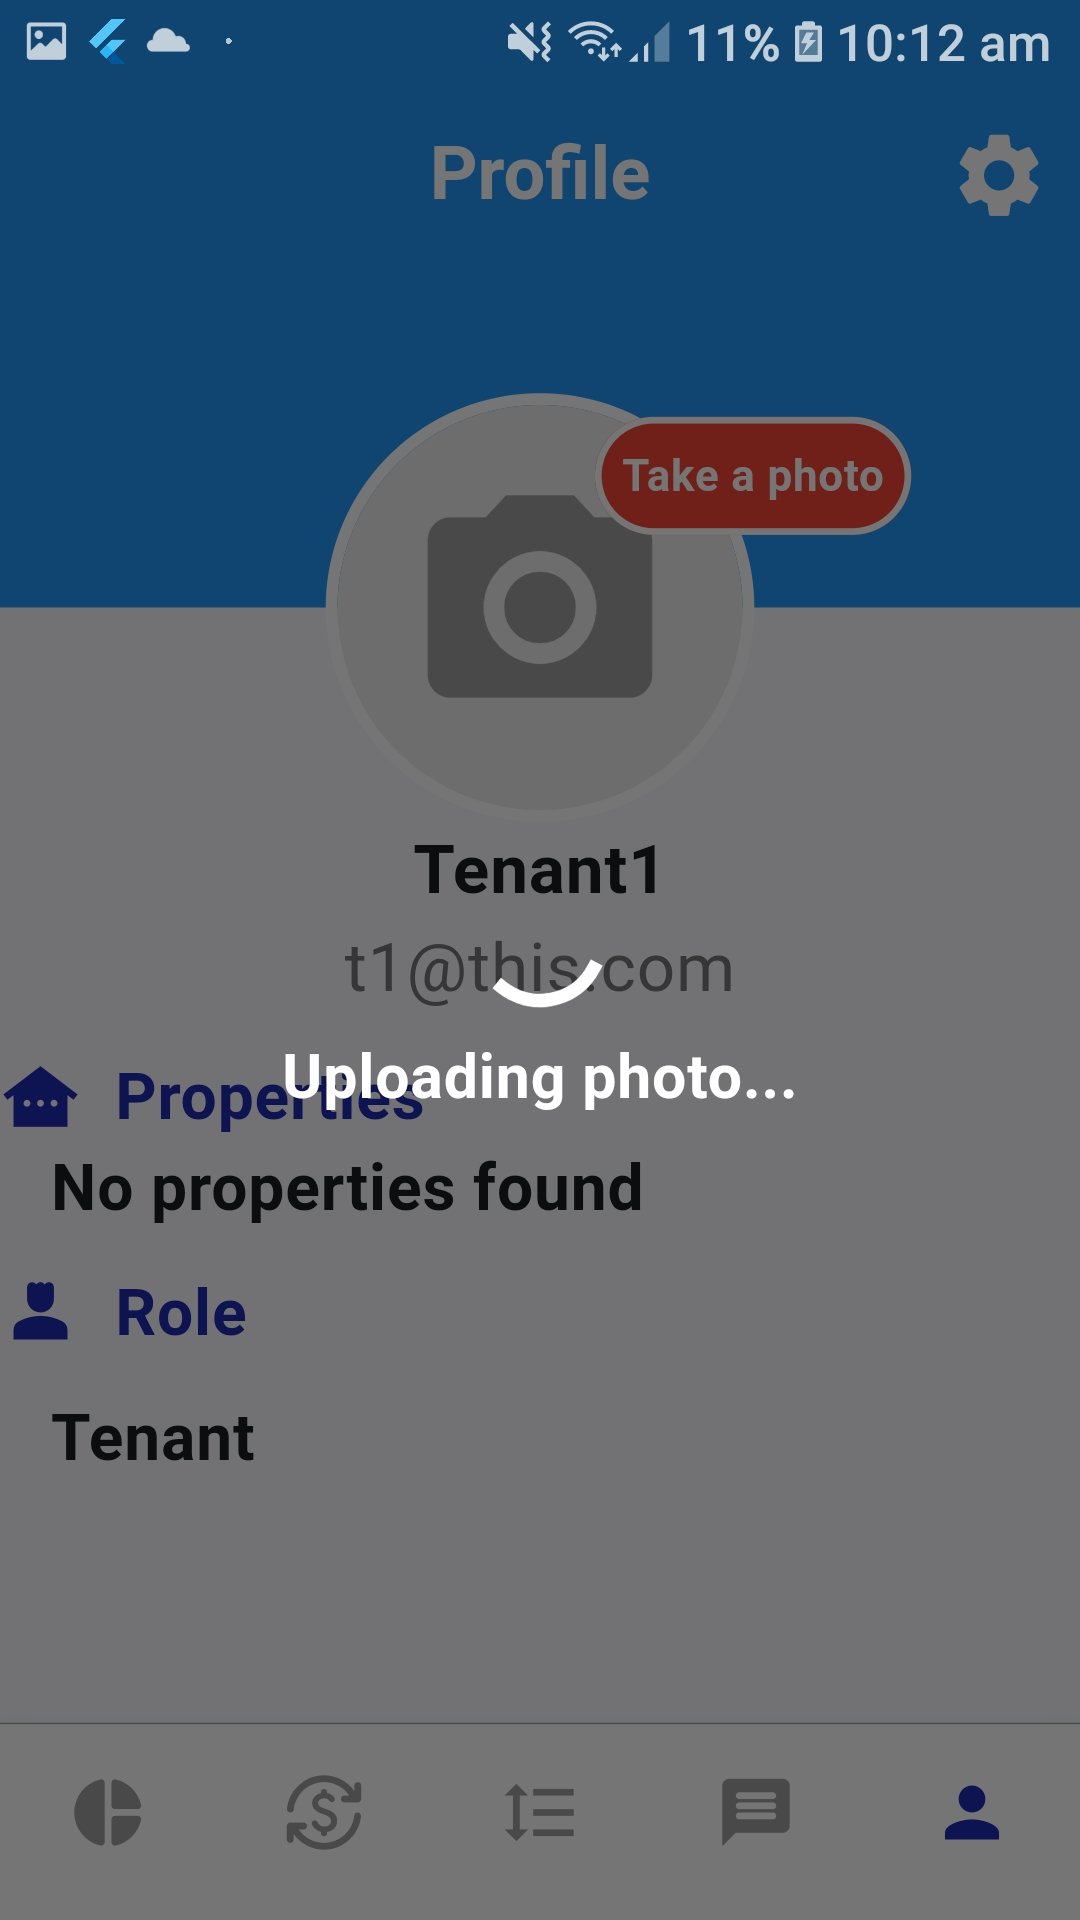
\includegraphics[width=0.24\textwidth]{faceCheckSuccess.jpg}
  \caption{Face Detected}
  \label{fig:faceCheckSuccess}
\end{figure}


\subsubsection{Text Recognition}
The text recognition feature allows landlords to take a photo of their bills, and the application will automatically extract the information from the photo and save it to the Cloud server for bill splitting. The text recognition function uses \specialterm{Google's ML Kit Text Recognition} SDK to extract text from the image (Figure~\ref{fig:beforeBillRecognition}). When the text is successfully recognised, the application will display the extracted information to the user (Figure~\ref{fig:billRecognitionDone}) in green. Accordingly, the upload button becomes clickable and turn green. This feature saves time and effort for landlords and ensures accurate data entry for bill splitting.

\begin{figure}[h]
  \centering
  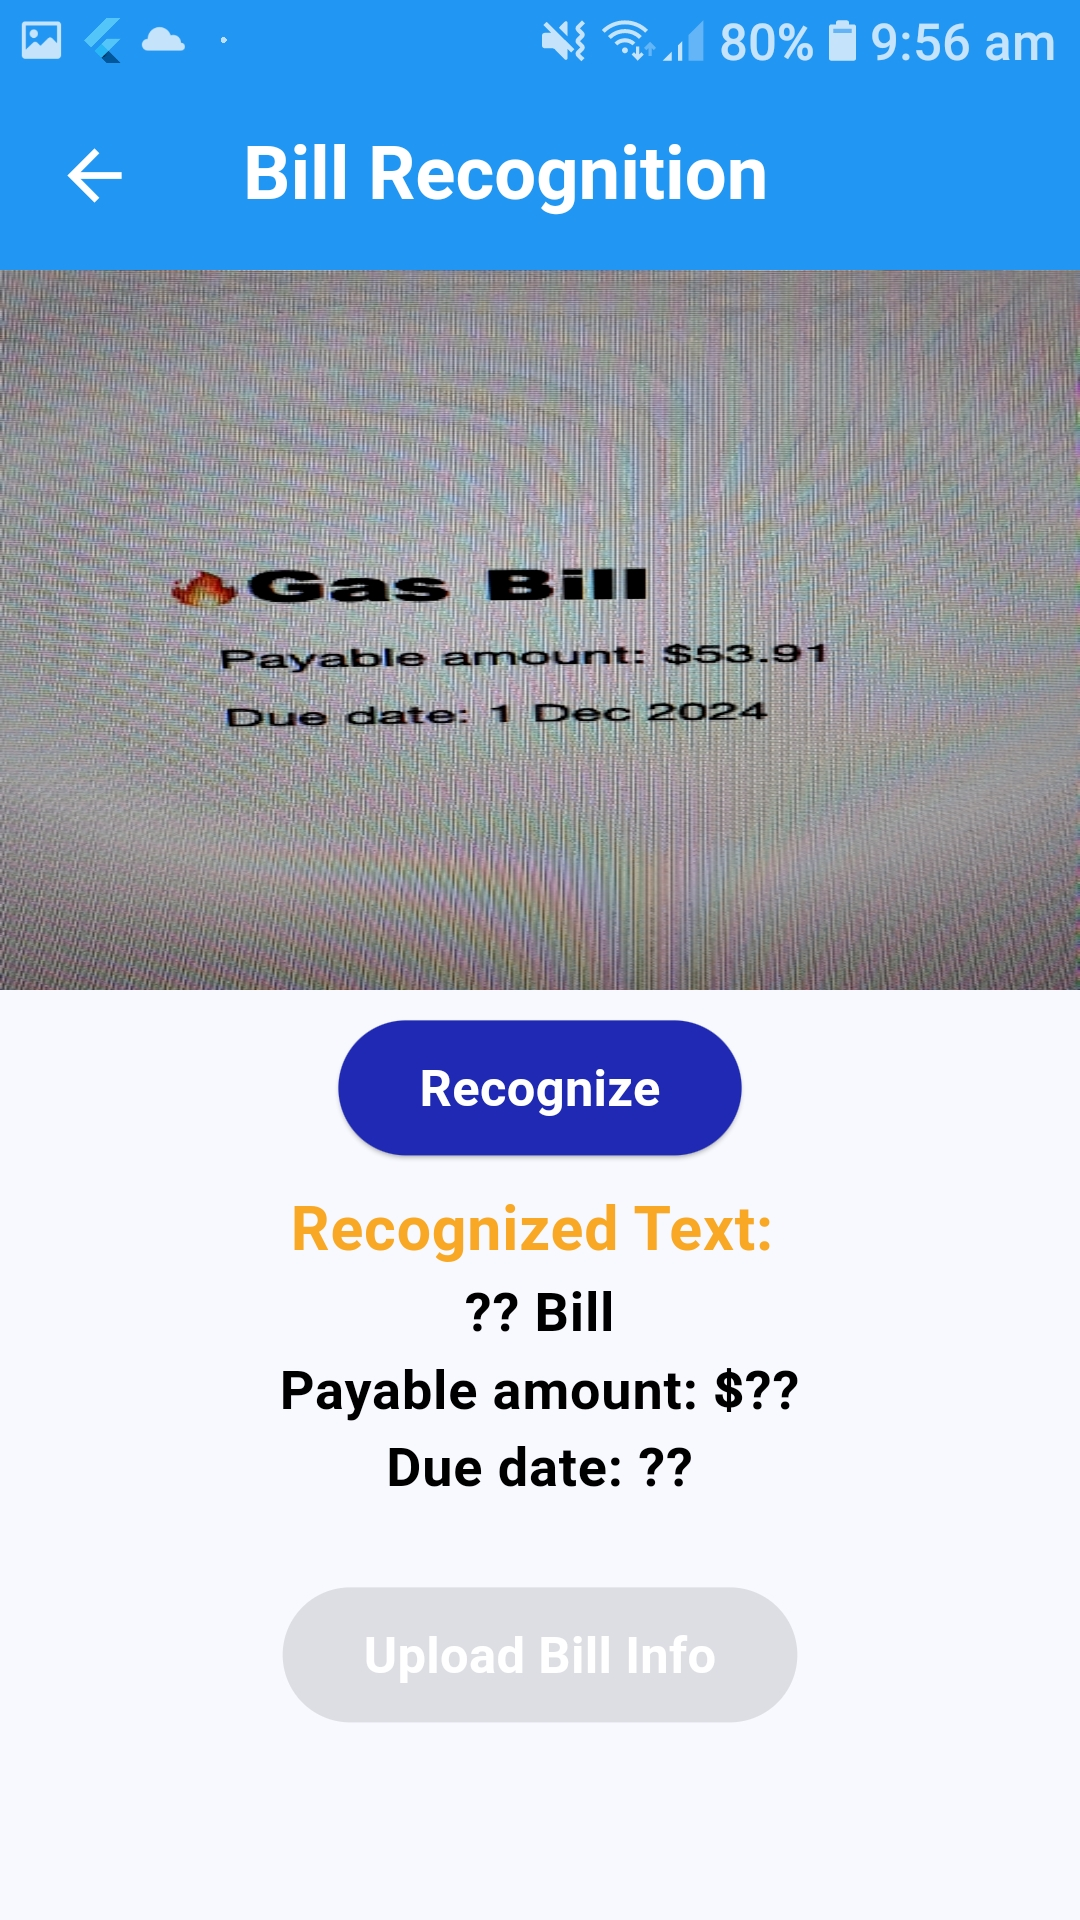
\includegraphics[width=0.24\textwidth]{beforeBillRecognition.jpg}
  \caption{Before Recognition}
  \label{fig:beforeBillRecognition}
\end{figure}
\begin{figure}[h]
  \centering
  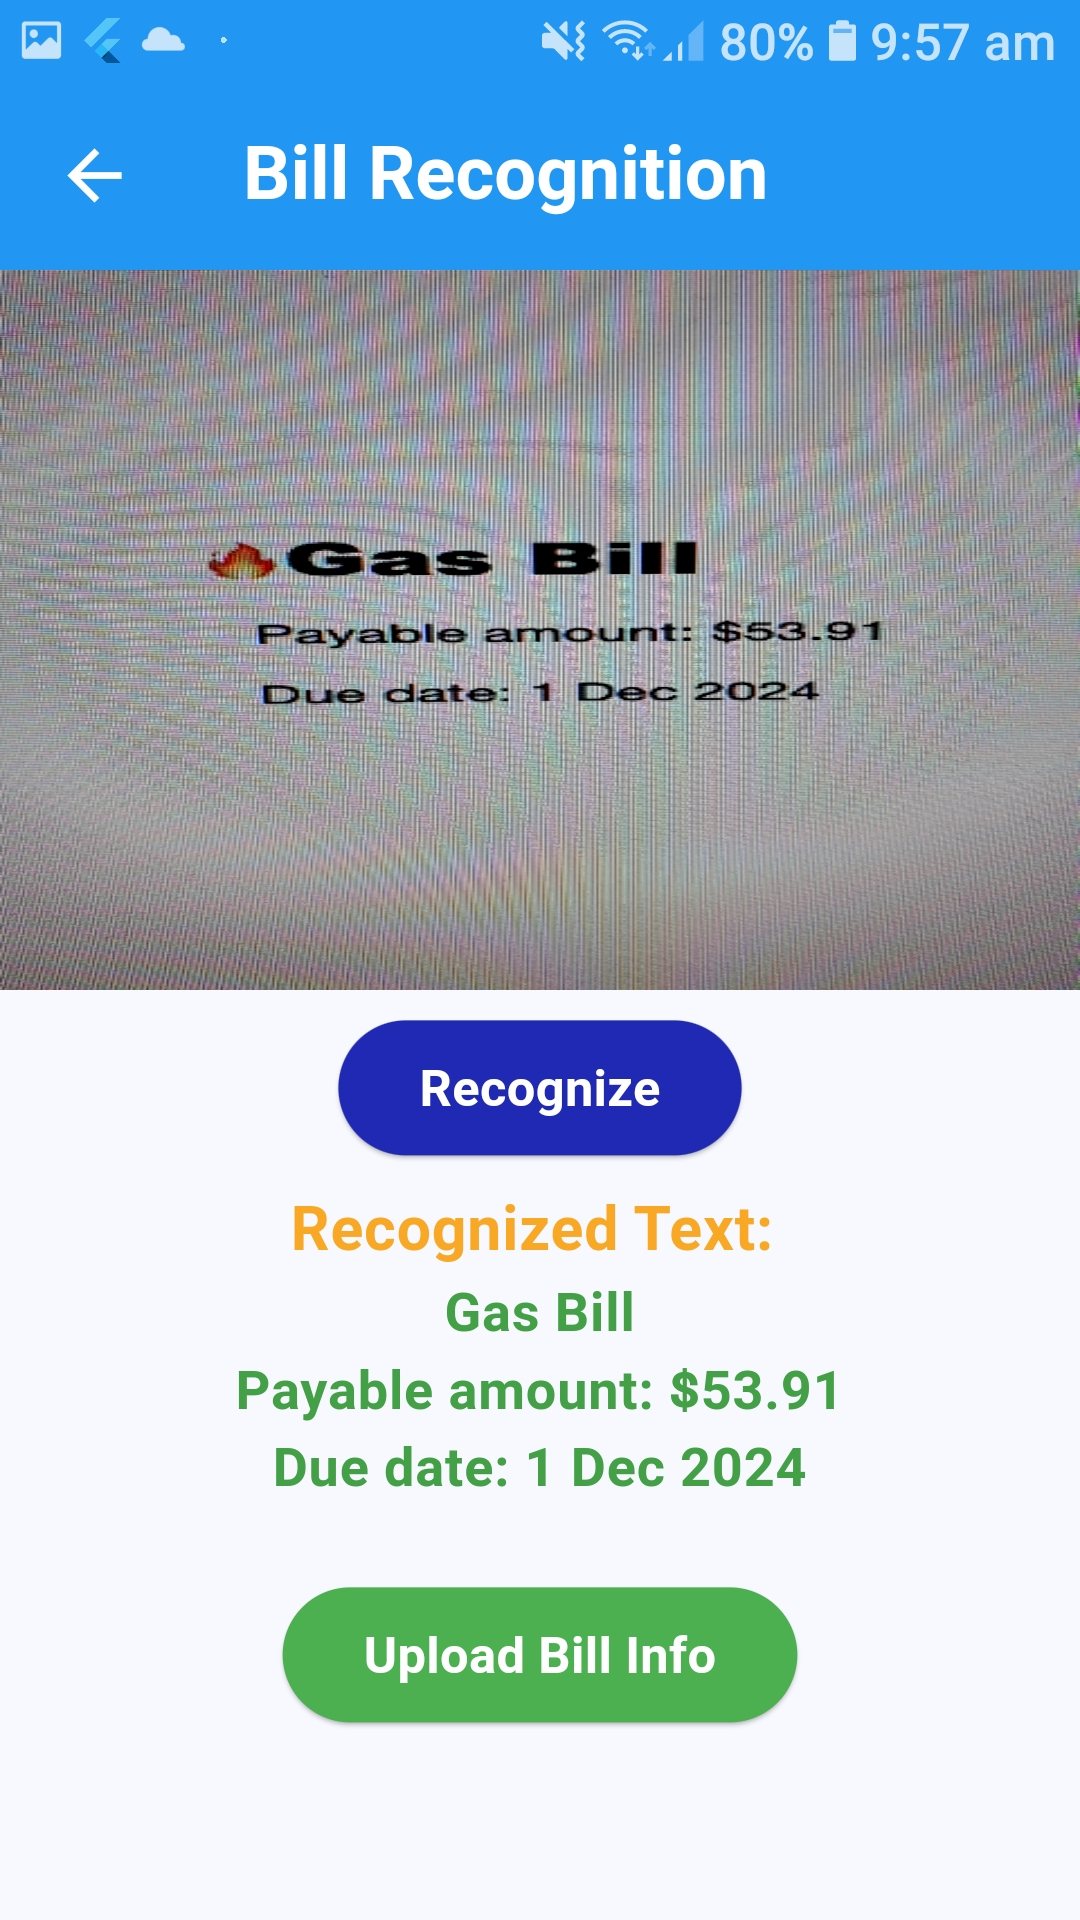
\includegraphics[width=0.24\textwidth]{billRecognitionDone.jpg}
  \caption{Successful Recognition}
  \label{fig:billRecognitionDone}
\end{figure}

\subsubsection{Usage Tracking}
The usage tracking function allows residents to view their usage data for different resources, such as electricity, water, Internet, and gas. The application displays the total usage durations for each resource in a day, a week, or a month (Figure~\ref{fig:usageOverview}). The usage data is presented in a graph format (Figure~\ref{fig:barChart}), making it easy for residents to understand their consumption patterns and identify areas where they can reduce their usage and save money.

\begin{figure}[h]
  \centering
  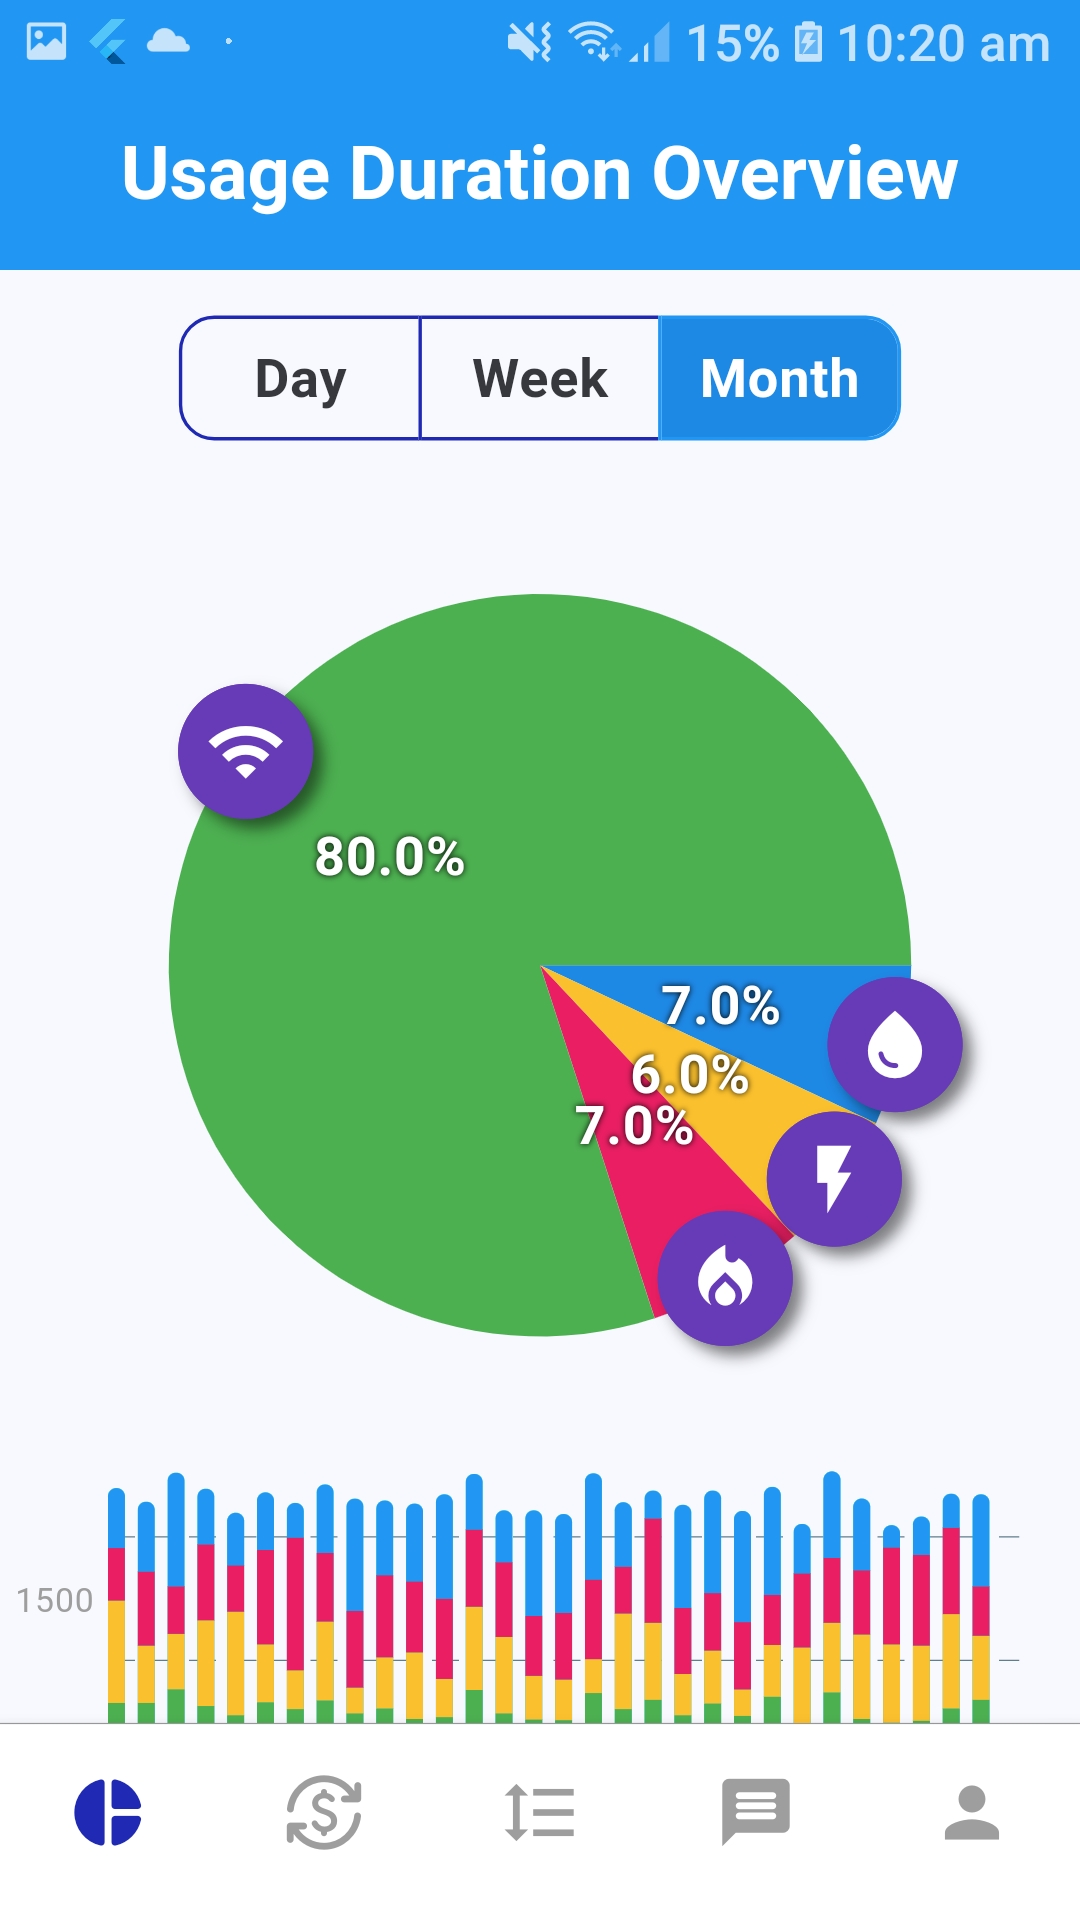
\includegraphics[width=0.25\textwidth]{pieChartOverview.jpg}
  \caption{Usage Overview}
  \label{fig:usageOverview}
\end{figure}
\begin{figure}[h]
  \centering
  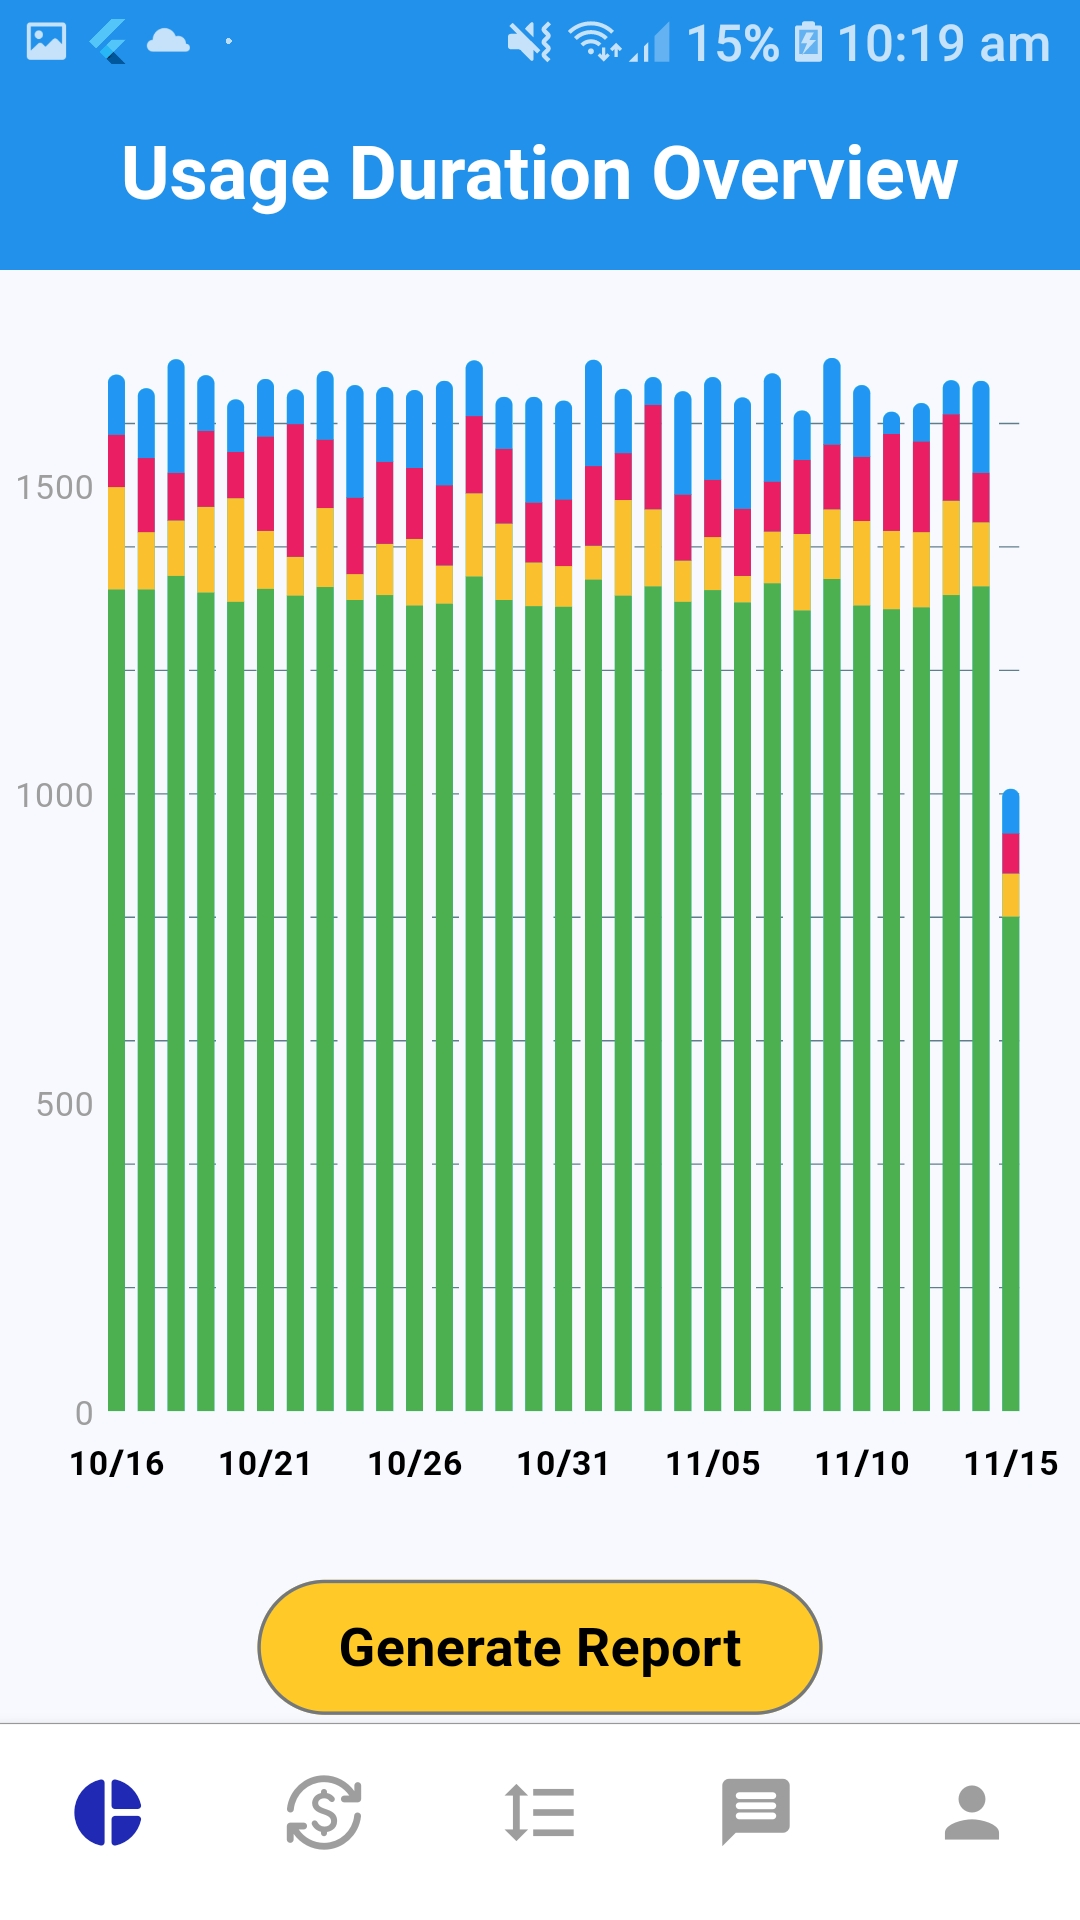
\includegraphics[width=0.26\textwidth]{30DayBarChart.jpg}
  \caption{Bar Chart Showing One-Month Usage}
  \label{fig:barChart}
\end{figure}

\subsubsection{Actions History}
The actions history is displayed in a continuous timeline interface. Residents can view their actions history, such as using WIFI, turning on the light, turning on the gas or faucet, etc. The timeline interface provides a visual representation of the residents' activities in a chronological order (Figure~\ref{fig:actionTimeline}). Residents can scroll through the timeline to view their past actions and identify any unusual patterns or activities. Landlords can also view the actions history of all residents to monitor their activities and ensure compliance with the house rules.

\begin{figure}[h]
  \centering
  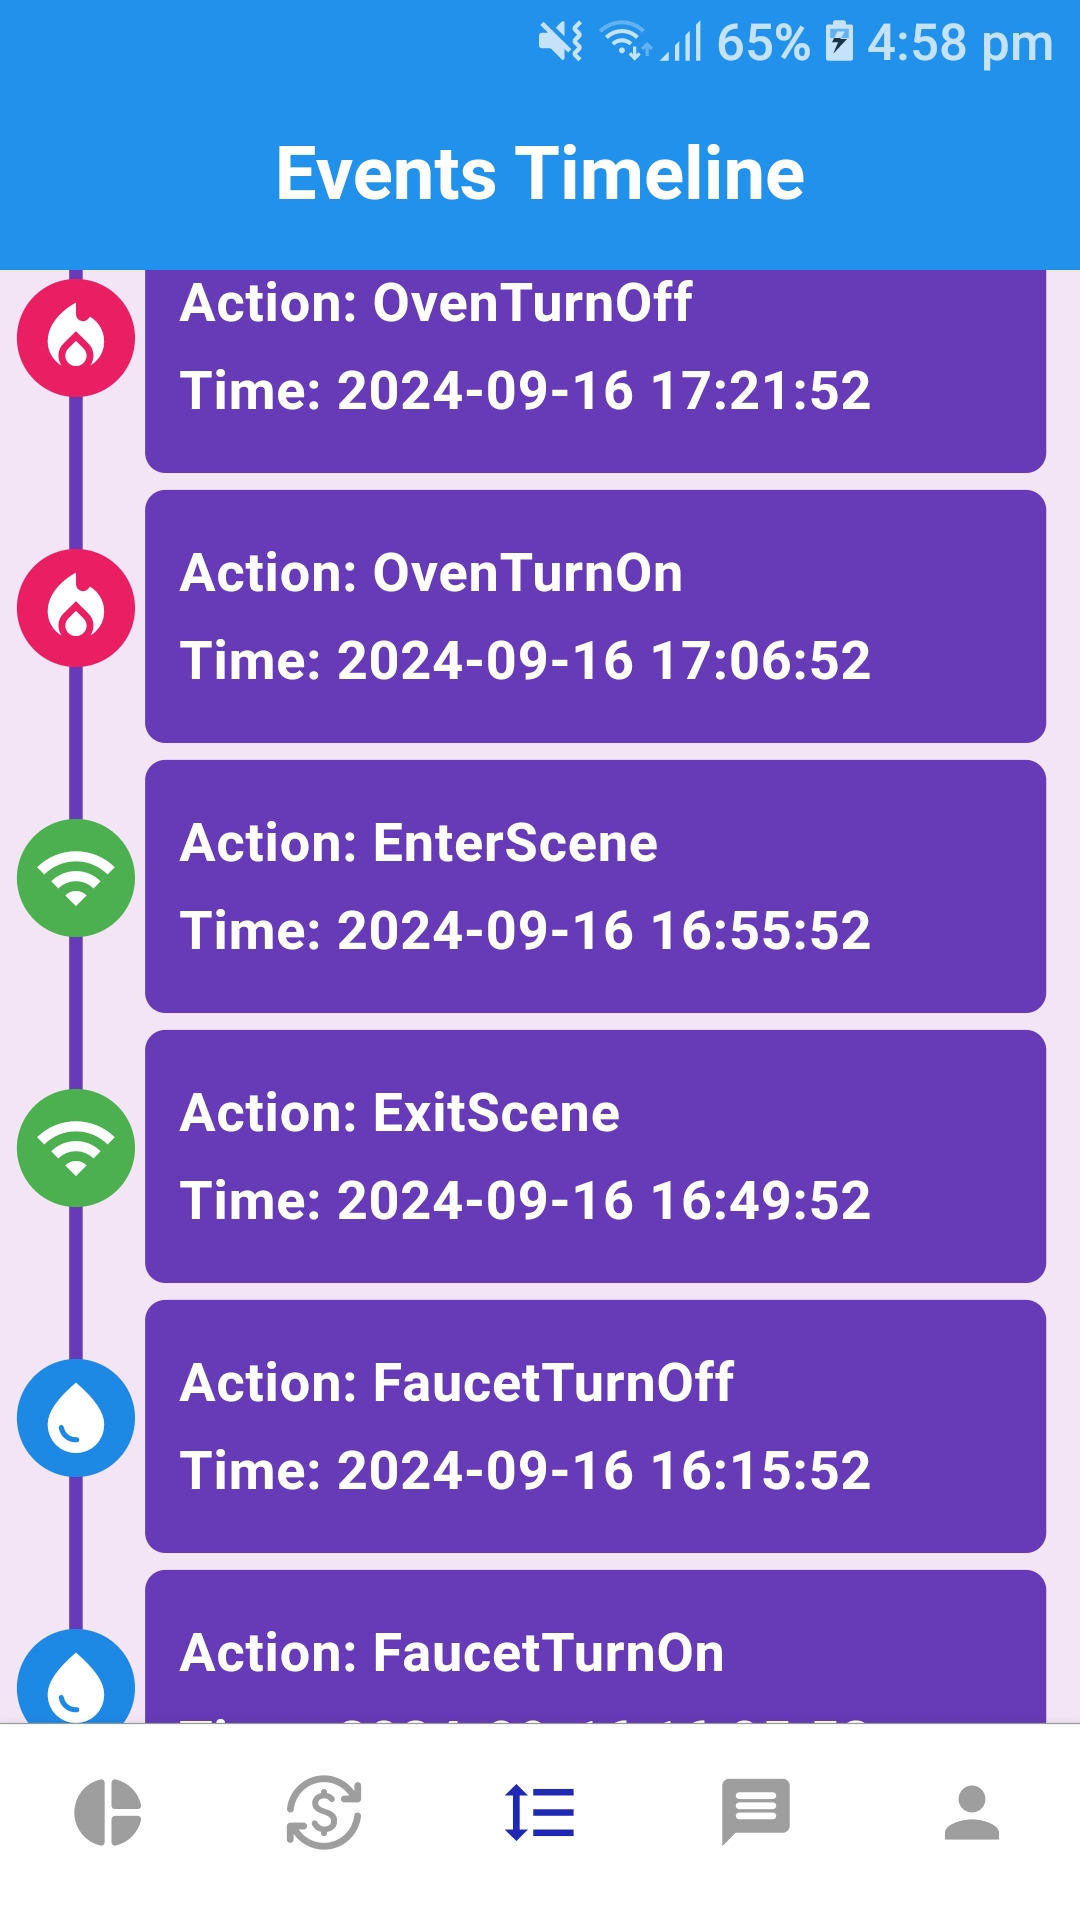
\includegraphics[width=0.24\textwidth]{actionTimeline.jpg}
  \caption{Events Timeline}
  \label{fig:actionTimeline}
\end{figure}

\subsubsection{Pay Bills}
Pay Bills page (Figure~\ref{fig:unpaidBills}) allows residents to query their unpaid bills and pay them through the application (no real money is involved, see Figure~\ref{fig:payBill}).

\begin{figure}[h]
  \centering
  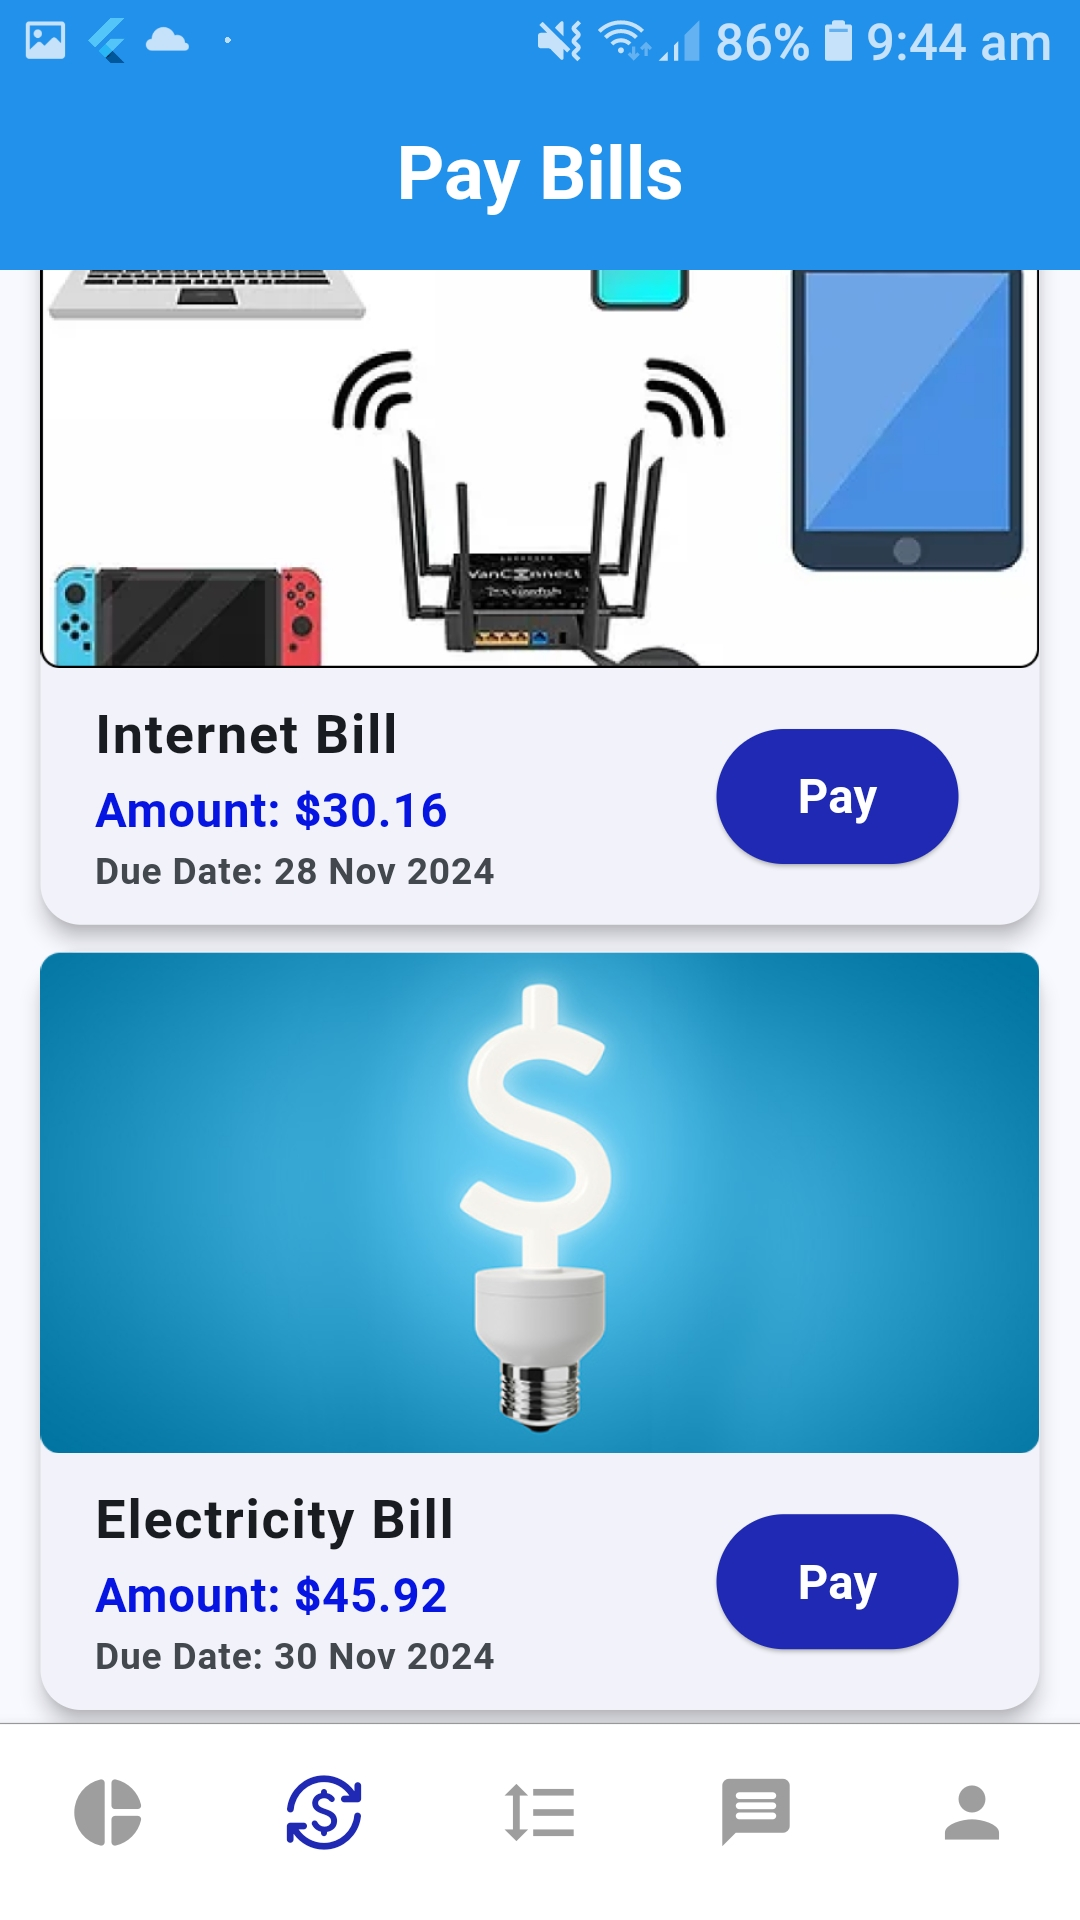
\includegraphics[width=0.24\textwidth]{unpaidBills.jpg}
  \caption{Pay Bills Page}
  \label{fig:unpaidBills}
\end{figure}
\begin{figure}[h]
  \centering
  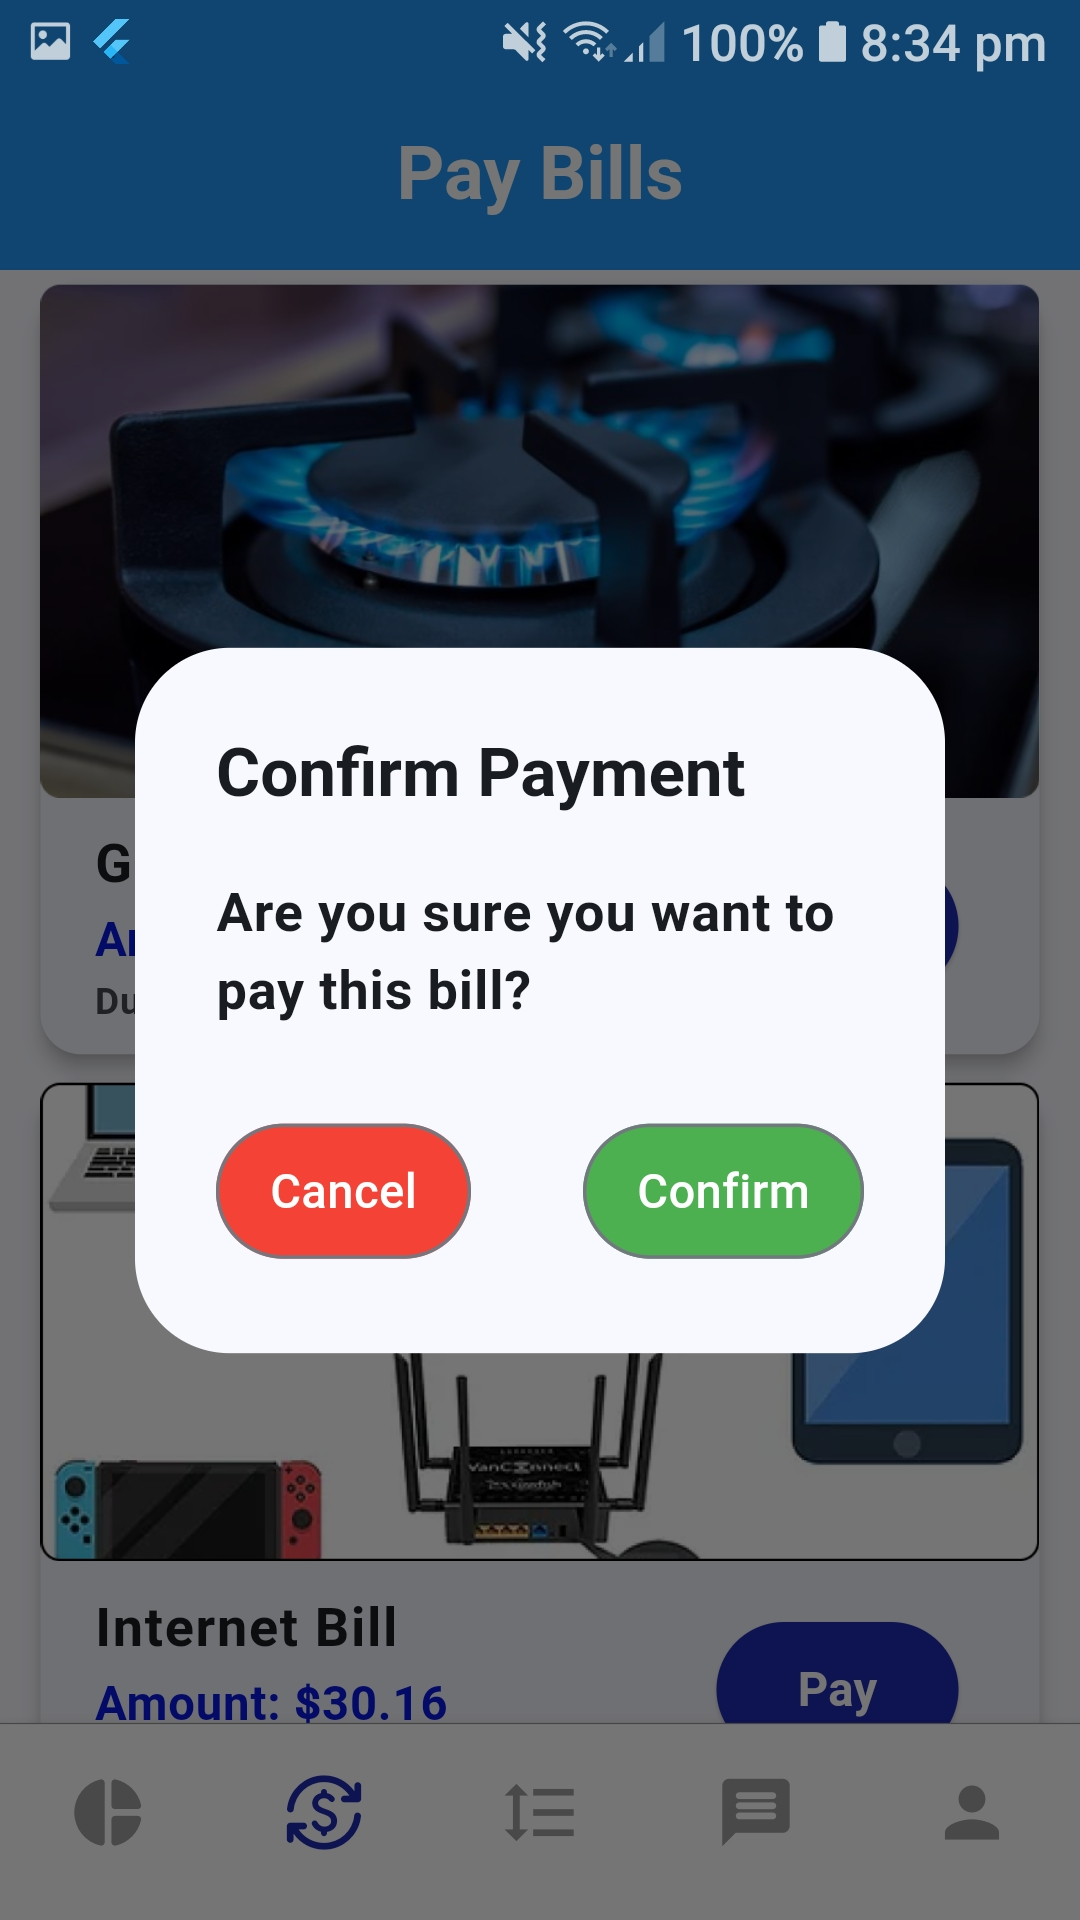
\includegraphics[width=0.24\textwidth]{payBill.jpg}
  \caption{Pay Bills}
  \label{fig:payBill}
\end{figure}

\subsubsection{Generate Report}
The generate report function allows residents to generate a report for their last 30-day usage data (Figure~\ref{fig:usageReport}). The report includes the total usage duration for each resource, daily usage patterns, and recommendations for reducing consumption and saving money. We implemented this by sending usage data to the API of OpenAI.\@ With proper prompt, it can return appropriate results.

\begin{figure}[h]
  \centering
  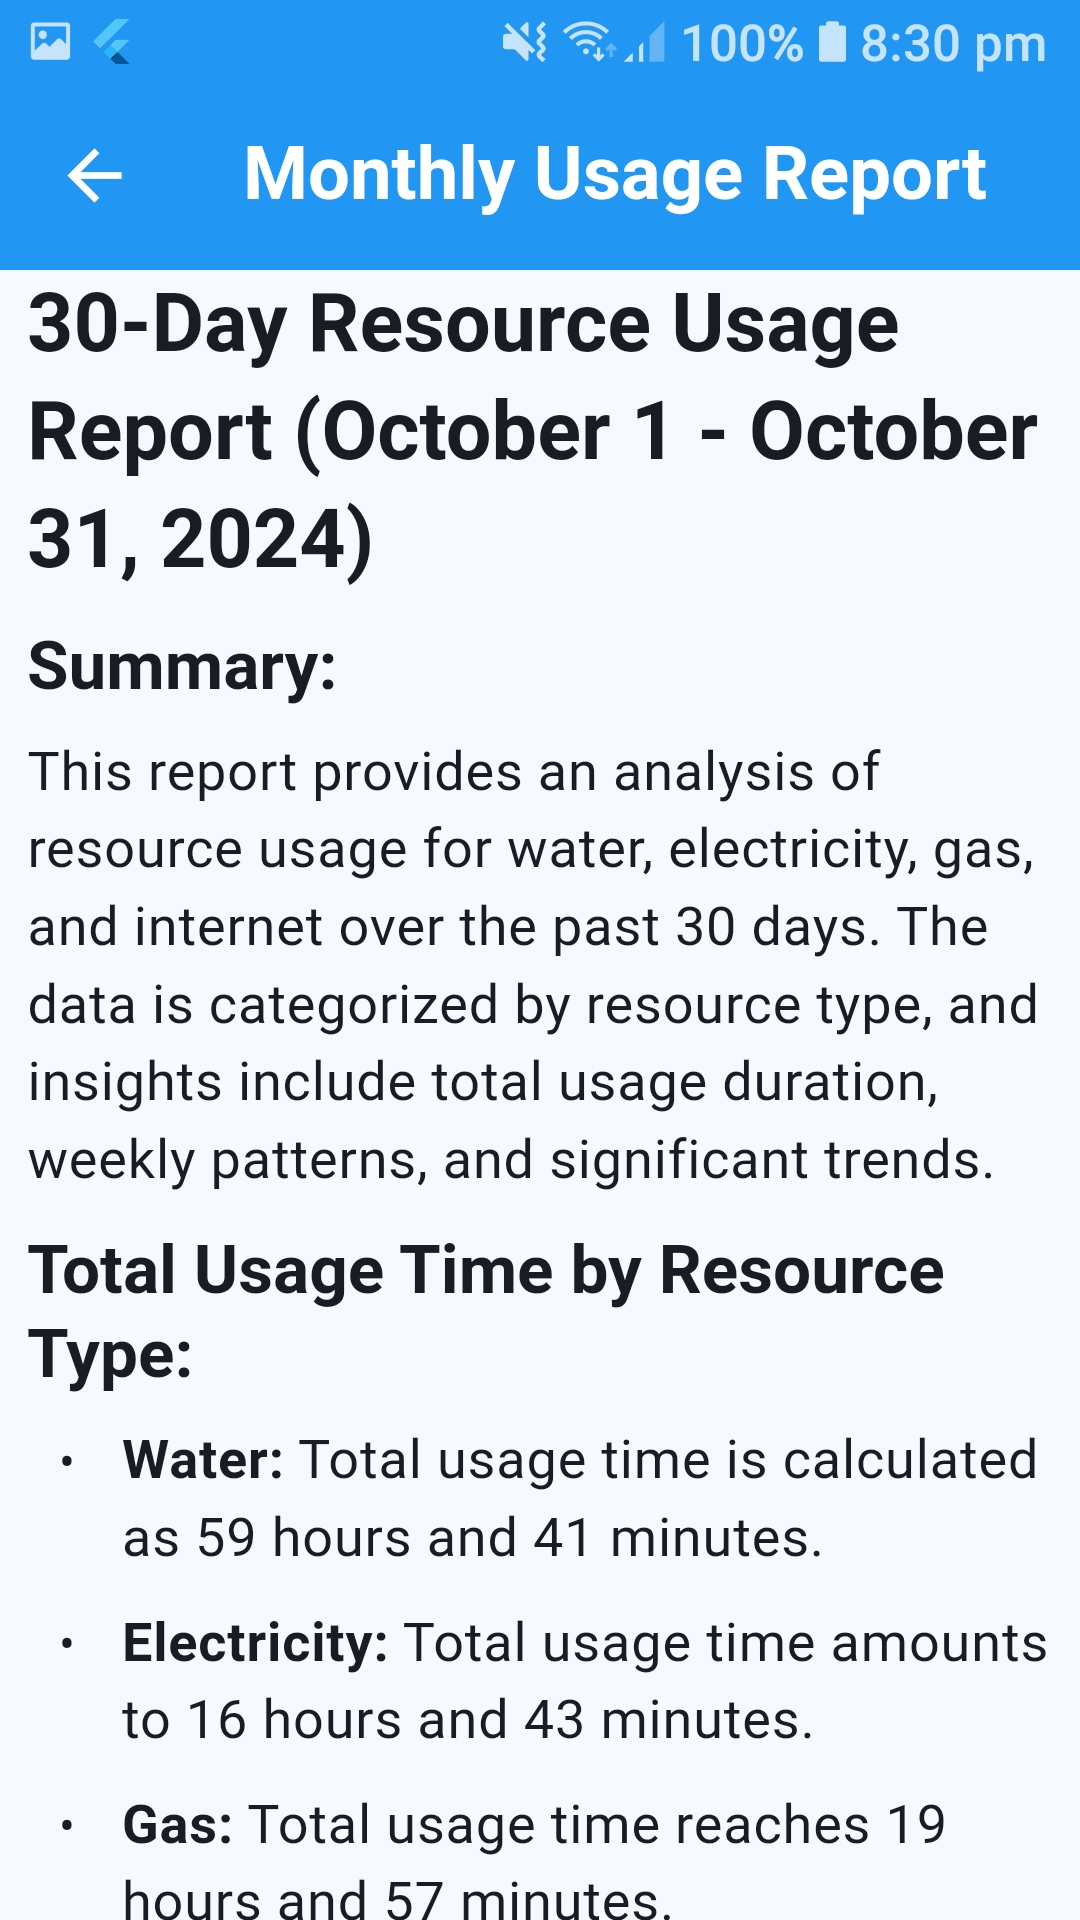
\includegraphics[width=0.24\textwidth]{usageReport.jpg}
  \caption{Monthly Usage Report}
  \label{fig:usageReport}
\end{figure}

\section{Evaluation}
Our SplitMateEZ Android application has been tested on two different models of Android phones, including Samsung Galaxy A5 and LG K4. The functionality, accuracy, and performance of the application were thoroughly evaluated, confirming that it meets expected standards. Residents benefit from a smooth experience as they access usage logs, make payments, and communicate with the landlord. The design prioritizes user-friendliness, with an intuitive layout and helpful prompts, ensuring ease of navigation. Responsiveness is optimal, with minimal lag, contributing to an efficient user experience. Data protection is achieved through encryption and authentication, guaranteeing security for user information. Reliability is demonstrated through stable performance, with minimal instances of crashes or freezes under normal usage conditions. Additionally, the application scales effectively to support numerous users and properties while remaining resource-efficient, without excessive battery or memory consumption.

\section{Conclusion}
The SplitMateEZ Android application offers a comprehensive solution for residents in shared accommodations to manage utility bills effectively. By leveraging advanced features such as face recognition, text recognition, and usage tracking, the application provides a user-friendly interface for residents to monitor their usage, receive notifications, and communicate with the landlord. The application has been rigorously tested and evaluated, demonstrating high performance, accuracy, and reliability. Residents can benefit from a seamless experience as they access their usage logs, pay bills, and generate reports, ensuring transparency and fairness in bill-splitting. The SplitMateEZ application represents a significant advancement in utility management for shared accommodations, offering a secure, efficient, and user-friendly solution for residents and landlords.

\section{Future Work}
In the future, we plan to further enhance the SplitMateEZ Android application by implementing additional features and improvements. These include: 1. use cache to store the data for enchance the speed of the application; 2. implement a feature that allows residents to set usage limits for each resource and receive notifications when they exceed the limits; 3. integrate the application with smart home devices to enable landlords to remotely control resource areas and monitor residents' activities; 4. add video streaming feature to allow residents to view live feeds from security cameras and monitor their property remotely; 5. implement a feature that allows residents to report maintenance issues and request repairs through the application; 6. integrate the application with payment gateways to enable residents to pay their bills directly through the application; 7. add a feature that allows residents to view their usage data in comparison to other residents in the same property or in other properties; 8. integrate the application with social media platforms to enable residents to share their usage data and insights with their friends and family.


%%
%% The next two lines define the bibliography style to be used, and
%% the bibliography file.
\newpage
\bibliographystyle{ACM-Reference-Format}
\bibliography{sample-base}


%%
%% If your work has an appendix, this is the place to put it.
\appendix

\section{Research Methods}

\subsection{Part One}

Lorem ipsum dolor sit amet, consectetur adipiscing elit. Morbi
malesuada, quam in pulvinar varius, metus nunc fermentum urna, id
sollicitudin purus odio sit amet enim. Aliquam ullamcorper eu ipsum
vel mollis. Curabitur quis dictum nisl. Phasellus vel semper risus, et
lacinia dolor. Integer ultricies commodo sem nec semper.

\subsection{Part Two}

Etiam commodo feugiat nisl pulvinar pellentesque. Etiam auctor sodales
ligula, non varius nibh pulvinar semper. Suspendisse nec lectus non
ipsum convallis congue hendrerit vitae sapien. Donec at laoreet
eros. Vivamus non purus placerat, scelerisque diam eu, cursus
ante. Etiam aliquam tortor auctor efficitur mattis.

\section{Online Resources}

Nam id fermentum dui. Suspendisse sagittis tortor a nulla mollis, in
pulvinar ex pretium. Sed interdum orci quis metus euismod, et sagittis
enim maximus. Vestibulum gravida massa ut felis suscipit
congue. Quisque mattis elit a risus ultrices commodo venenatis eget
dui. Etiam sagittis eleifend elementum.

Nam interdum magna at lectus dignissim, ac dignissim lorem
rhoncus. Maecenas eu arcu ac neque placerat aliquam. Nunc pulvinar
massa et mattis lacinia.

\end{document}
\endinput
%%
%% End of file `sample-sigconf.tex'.
